\documentclass[article,shortnames, nojss]{jss}

%\VignetteIndexEntry{Robust Tools for Three-way Component Analysis of Compositional Data: The R package rrcov3way}
%\VignetteKeywords{robustness, multi-way analysis, PARAFAC, TUCKER3}
%\VignettePackage{rrcov3way}

\usepackage[ansinew]{inputenc}
\usepackage{multirow}
\usepackage{color}
\usepackage{mathtools}
\usepackage{fixltx2e}
\usepackage{float}
\floatplacement{figure}{H}

\usepackage{amsmath}                %% need for subequations
\usepackage{amssymb}
\usepackage{amsfonts}
\usepackage{hyperref}
\usepackage[english]{babel}

%%%%%%%%%%%%%%%%%%%%%%%%%%%%%%
%% declarations for jss.cls %%%%%%%%%%%%%%%%%%%%%%%%%%%%%%%%%%%%%%%%%%
%%%%%%%%%%%%%%%%%%%%%%%%%%%%%%
\newcommand{\vv}[1]{\mbox{\boldmath$#1$}}
\newcommand{\xv}{\mbox{\boldmath$x$}}
\newcommand{\yv}{\mbox{\boldmath$y$}}
\newcommand{\zv}{\mbox{\boldmath$z$}}
\newcommand{\mv}{\mbox{\boldmath$m$}}
\newcommand{\tv}{\mbox{\boldmath$t$}}
\newcommand{\xbarv}{\mbox{\boldmath$\bar x$}}
\newcommand{\uv}{\mbox{\boldmath$u$}}
\newcommand{\muv}{\mbox{\boldmath$\mu$}}
\newcommand{\nuv}{\mbox{\boldmath$\nu$}}
\newcommand{\deltav}{\mbox{\boldmath$\delta$}}
\newcommand{\chiv}{\mbox{\boldmath$\chi$}}
\newcommand{\ov}{\mbox{\boldmath$0$}}

\newcommand\MCD{\mathit{MCD}}
\newcommand\MVE{\mathit{MVE}}
\newcommand\OGK{\mathit{OGK}}
\newcommand\diag{\mathrm{diag}}
%\newcommand\det{\mathrm{det}}

\newcommand{\R}{\textbf{\textsf{R}}}
\newcommand{\class}[1]{``\code{#1}''}
\newcommand{\fct}[1]{\code{#1()}}

%% almost as usual
%% almost as usual
\author{Valentin Todorov\\UNIDO \And
        Violetta Simonacci\\University of Naples-L'Orientale \AND
        Maria Anna Di Palma\\University of Naples-L'Orientale \AND Michele Gallo\\University of Naples-L'Orientale}

\title{Robust Tools for Three-way Component Analysis of Compositional Data: The \proglang{R} package \pkg{rrcov3way}}

%% for pretty printing and a nice hypersummary also set:
\Plainauthor{Valentin Todorov, Violetta Simonacci, Maria Anna Di Palma, Michele Gallo} %% comma-separated
\Plaintitle{rrcov3way: An R Package for Robust Three-way Analysis}   %% without formatting
%% \Shorttitle{R package for three-way analysis} %% a short title (if necessary)

\Abstract{
The \proglang{R} package \pkg{rrcov3way} provides a set of tools for fitting the Tucker3 and PARAFAC models to multidimensional arrays by use of classical, robust and compositional estimating procedures. Two main functions are implemented, Parafac and Tucker3, which include alternative options to the standard least squares algorithm in order to properly calculate the models in case of data with outliers and/or characterized by a biased covariance structure. A comprehensive collection of three-way plots, diagnostics and data processing functions is also made available.
A brief overview of multilinear tools, robustification procedures and compositional data analysis for three-way arrays is followed by a detailed presentation on the use and applicability of the implemented functions by means of real data examples included in the package.}
\Keywords{Parafac, Tucker3, compositional data, closed data, log-ratio, robustness, outlier}
%%\Plainkeywords{Parafac, Tucker3, compositional data, closed data, log-ratio, robustness, outlier}

%% without formatting
%% at least one keyword must be supplied

%% publication information
%% NOTE: Typically, this can be left commented and will be filled out by the technical editor
%% \Volume{13}
%% \Issue{9}
%% \Month{September}
%% \Year{2004}
%% \Submitdate{2004-09-29}
%% \Acceptdate{2004-09-29}

%% The address of (at least) one author should be given
%% in the following format:
\Address{
  Valentin Todorov\\
  Department of Policy, Research and Statistics\\
  United Nations Industrial Development Organization (UNIDO)\\
  Vienna International Centre\\
  P.O.Box 300, 1400, Vienna, Austria\\
  E-mail: \email{valentin@todorov.at}\\
%  URL: \url{http://statmath.wu-wien.ac.at/~zeileis/}

    Violetta Simonacci\\
    Department of Human and Social Sciences\\
    L'Orientale--University of Naples\\
    P.zza S.Giovanni Maggiore, 30\\
    Naples, 80134, Italy\\
    E-mail:  \email{vsimonacci@unior.it}\\

    Maria Anna Di Palma\\
    Department of Human and Social Sciences\\
    LOrientale--University of Naples\\
    P.zza S.Giovanni Maggiore, 30\\
    Naples, 80134, Italy\\
    E-mail:  \email{madipalma@unior.it}\\

    Michele Gallo\\
    Department of Human and Social Sciences\\
    L'Orientale--University of Naples\\
    P.zza S.Giovanni Maggiore, 30\\
    Naples, 80134, Italy\\
    E-mail:  \email{mgallo@unior.it}\\
}
%% It is also possible to add a telephone and fax number
%% before the e-mail in the following format:
%% Telephone: +43/1/31336-5053
%% Fax: +43/1/31336-734

%% for those who use Sweave please include the following line (with % symbols):
%% need no \usepackage{Sweave.sty}

%% end of declarations %%%%%%%%%%%%%%%%%%%%%%%%%%%%%%%%%%%%%%%%%%%%%%%

\newcommand{\bi}{\begin{itemize}}
\newcommand{\ei}{\end{itemize}}
\newcommand{\be}{\begin{enumerate}}
\newcommand{\ee}{\end{enumerate}}
\renewcommand{\v}[1]{\mathbf{#1}}
%% Sweave options for the complete document
%%\SweaveOpts{keep.source=TRUE}



\graphicspath{{./images/}}


\begin{document}

%% include your article here, just as usual
%% Note that you should use the \pkg{}, \proglang{} and \code{} commands.

\section[Introduction]{Introduction}
\label{sec:intro}
The most usual way to start exploring data on $m$ objects in $p$
continuous variables is by principal component analysis (PCA). This procedure
summarizes the most important information in the data by representing
the objects and the variables simultaneously by a limited number
of optimally selected components. The optimality
of these components is intended in the sense that they explain the
maximal possible variance. The components remain optimal
even after rotation, thus, it is possible to search for a structure
which allows for easier interpretation. If these data are
measured at $k$ occasions (conditions, times, locations),
generalizations of PCA, that can handle three-way data, are needed. The first such
generalization that comes at hand is PARAFAC (parallel
factor analysis), alternatively called CANDECOMP
(canonical decomposition)\citep{Harshman:1970, Carroll:1970}.
PARAFAC summarizes
simultaneously the objects, variables and occasions in an optimally
selected lower dimensional (with a limited number of components)
representation. The solution provided by PARAFAC is unique, i.e.,
it does not allow for rotation.
Another popular trilinear
decomposition method is the Tucker3 model which was suggested
already in 1966 by \citet{Tucker:1966} for solving three-way
problems in the field of psychometrics. The decomposition provided by
the Tucker3 model results into a core array and three eigenvector
matrices. In contrast to the PARAFAC model, the solution provided
by Tucker3 is not unique. Any arbitrary nonsingular rotation of
all components simultaneously will retain the model representation, producing a new solution.\\\\
While in the rest of this paper we will limit the discussion to
three-way data, it is obvious that extension to higher orders
is straightforward. With the nowadays advanced data capture methods
in across a variety of applications, producing complex data structures,
multiway methods with their ability to uncover the underlying
structures, gained wide popularity. Originating in psychometrics
these models are now applied in chemometrics, social networks,
process control, econometrics. This resulted into a large
number of publications, see \citet{acar:2009} for a review.
\citet{kroonenberg:2016} provides a very personal view on
the development and the recent status of multiway analysis.\\\\
To make the models readily available for practical use, a number of
software tools were developed, particularly in \proglang{MATLAB}
with the most comprehensive package being
the \pkg{NWay} toolbox \citep{bro:2000}. A graphical interface to \pkg{NWay}
is provided by \pkg{CuBatch} \citep{cubatch:2005}. The robust version of PARAFAC
introduced by \citet{Engelen11} is provided in the \proglang{MATLAB} toolbox for
robust statistics \pkg{LIBRA} \citep{verboven-libra:2010}. Currently
several \proglang{R} packages are available at CRAN:
\pkg{PTAk} of \citet{leibovici:2010}, \pkg{ThreeWay} of \citet{threeway:2014},
\pkg{multiway} of \citet{multiway:2016} and \pkg{rTensor} of \citet{rTensor:2018}.
In this work another package for three-way modeling is presented, the package
\pkg{rrcov3way}, which aims to introduce additional tools not yet available
in \proglang{R}. Specifically its content responds to the need for flexible
functions suited for appropriately dealing with problematic features such
as the presence of outliers and/or of a compositional structure in the data.
The standard Tucker3 and PARAFAC estimating procedure, alternating least
squares (ALS), is extremely sensitive to the presence of anomalous observations,
which may artificially inflate the variance and skew the model away
from the real underlying solution.
For these reasons robust alternatives to classical PARAFAC and
Tucker3 models have been proposed. A robust version of Tucker3
based on the use of the minimum covariance determinant (MCD)
estimator \citep{Rousseeuw99} was introduced by \citet{pravdova2001robust}.
Later on \citet{Engelen11} extended this methodology to the PARAFAC
model by also revealing and correcting some of its inefficiencies. These
inefficiencies were corrected also for the robust version of Tucker3 model
by \cite{todorov:tucker3} and at the same time a version for handling
compositional data was proposed.
The robust functions provided in \pkg{rrcov3way} for both
Tucker3 and PARAFAC follow these two latter approaches.\\\\
Modeling compositional data also requires special tools. Compositions or CoDa (compositional data) are positive vectors that carry relative information and can be expressed as proportions of a whole. The elements of such vectors are bounded by an explicit or implicit sum constraint, which imposes a negative covariance bias and contradicts the typical assumptions of classical multivariate statistics. Geometrically, this constraint translates into compositions having one redundant dimension, therefore they are constricted in a subset of real space defined as simplex, characterized by a specific geometry called Aitchison geometry \citep{Ego05,Ego06,Ego03,egozcue2011elements}.
Standard models are designed to work without any bias within a Euclidean framework \citep{PawEgo,Bill01} and would return distorted results on compositions.
The preferred strategy for modeling CoDa is to project them onto Euclidean space by means of a transformation into log-ratio coordinates. Successively, classical analysis can be executed while results must  be interpreted in compositional terms.
When the row vectors of a three-way array are compositional in nature, i.e., observations are expressed as the proportion of a total recorded at several occasions, this approach must be followed before trilinear models can be fitted to the data. For this reason, compositional versions of the Tucker3 and PARAFAC models based on log-ratios were developed. For details see \citet{gallo:2015, gallo:2013, Engle13}. Recently, a robust version of the PARAFAC model for compositions was also developed in \citet{dipalma:2018}. These compositional and robust-compositional variants of classical trilinear models are made available in the \pkg{rrcov3way} package. \\\\
In brief, the main purpose of this work is to illustrate the unique tools introduced in the \proglang{R} package \pkg{rrcov3way} for modeling three-way data and three-way compositions with or without outliers. This is achieved by demonstrating through real data examples the relevance and correct use of the standard, robust, compositional and compositional-robust procedures included in the package and of other functions provided for the proper treatment and representation of results. In detail, the paper is organized in the following manner. In Section~\ref{sec:why} the innovative features of the \pkg{rrcov3way} package with respect to other existing packages in \proglang{R} and \proglang{MATLAB} are illustrated. In Section~\ref{sec:theory} the theoretical background is introduced by recalling some basic notions of standard trilinear models, robust procedures and compositional data analysis for three-way data. Section~\ref{sec:ex-intro} presents a quick ``getting started'' example demonstrating main functions and necessary steps for a complete three-way data analysis. For this purpose the \emph{OECD Electronics Industries Data} from \citet{kroonenberg:2008} are used. As it is usual in developing \proglang{R} packages, \pkg{rrcov3way} contains many example data sets which can be used to illustrate different features of the considered methodology. Examples based on several of these data sets are presented in Section~\ref{sec:examples}. Finally, Section~\ref{sec:conclusions} concludes with a  discussion of the package features, its limitations and the possible further extensions.


\section{Why do we need rrcov3way?}
\label{sec:why}
In the previous section the main \proglang{R} packages for the analysis of three-way
arrays were recalled, namely \pkg{PTak}, \pkg{ThreeWay}, \pkg{multiway} and
\pkg{rTensor}. They all implement general functions for carrying out
standard models, but at the same, by focusing on specific modeling
needs, they also provide different tools to the community. The \pkg{PTak}
package aims to deal with the modeling of data characterized by a
spatio-temporal context. It introduces the multidimensional method
Principal Tensor Analysis on k-Modes, but it also provides standard
PARAFAC and Tucker3 functions. There are, however, some limitations
on the minimal number of components which can be extracted. This package
also offers the advantage of providing procedures which support
non-identity metrics and penalization.
The \pkg{ThreeWay} package provides a more complete suite of functions
for modeling three-way data. Here the emphasis is on the PARAFAC and
Tucker3 models. The main functions are also available as interactive
tools which guide the user step by step into the analysis, offering
the possibility to choose constraints, pre-processing and post-processing
alternatives. Other useful features include basic plotting tools and
the possibility to obtain bootstrap percentile intervals.
The \pkg{multiway} package, on the other hand, concentrates on the
generalization of component models to $n$-dimensional arrays, in
addition it offers the option to impose non-negativity constraints
and provides other functions such as \emph{Individual Differences Scaling},
\emph{Multiway Covariates Regression} and \emph{Simultaneous Component Analysis}.
Lastly, the \pkg{rTensor} package, offers a framework for handling
and analyzing $n$-th order tensors by providing the S4 class \code{Tensor}
and common tensor operations and decompositions, including the
PARAFAC/CANDECOMP decomposition, Generalized Low Rank Approximations of Matrices,
Multilinear Principal Component Analysis, Population Value Decomposition
and all Tucker models. The $t$-product and the $t$-singular value
decomposition are also implemented for three-mode cases.\\\\
It is clear that none of the existing \proglang{R} packages provides
robust versions of standard decompositions for dealing with
three-way data contaminated by outliers. Such tools are available
only in \proglang{MATLAB}.
Here the \pkg{LIBRA} package implements a robust PARAFAC model while
the \pkg{CuBatch} interface allows for outliers identification analysis
by providing an advanced version of the \pkg{NWay} toolbox,
a compendium of all multi-way functions in the environment.
In this perspective the first important contribution of the
\pkg{rrcov3way} package is to integrate the classical functions
for the decomposition of three-mode data with robust tools. Moreover it adds
another advanced feature which none of the above packages provides:
multi-way modeling of compositional data. Like other statistical tools,
the PARAFAC and Tucker3 models cannot be applied directly to compositions
due to the spurious correlations issue, therefore a specific methodology
must be followed. The attention on compositional data analysis has
increased in the past years and its usage has spread to various
disciplines such as chemistry, geosciences, biology, agriculture,
but also human and behavioral sciences. This increase in applicability
is also due to the broadening of the concept of composition, which
now also included implicit sum constraints and problems with both
dimensional and relative aspects \citep{pawlowsky2015modeling, pawlowsky2015tools}.
Tailoring standard multilinear tools to this methodology can, thus,
prove of great interest. For this reason an option to carry out a
compositional version of model functions is included in the package.
Specifically, the included \code{Parafac()} and \code{Tucker3()} functions present the
option of carrying out four different types of analysis by means of
two parameters, \code{robust=TRUE/FALSE} and \code{coda.transform="none"}
(default) or \code{coda.transform="ilr"}:
\begin{enumerate}
\item Classical Analysis: the model is estimated on the original array
    entries (with or without standard preprocessing) using the alternating
    least square (ALS) algorithm (\code{robust=FALSE, coda.transform="none"});
\item Robust Analysis: the original array is robustified and then the
    ALS algorithm is performed. Outliers are identified and accommodated
    without affecting the solution  (\code{robust=TRUE, coda.transform="none"});
\item Compositional Analysis: data are transformed in log-ratio coordinates,
    the ALS algorithm is performed and the output is expressed in
    log-contrasts  (\code{robust=FALSE, coda.transform="ilr" or coda.transform="clr"});
\item Robust and Compositional Analysis: data are first expressed in
    log-ratio coordinates, then the transformed array is robustified and
    ultimately the ALS algorithm is performed  (\code{robust=TRUE, coda.transform="ilr"}).
\end{enumerate}
These four types of analysis are provided in \pkg{rrcov3way} for both PARAFAC
and Tucker3 models. Compared to the other existing software packages, \pkg{ThreeWay} and
the other already mentioned \proglang{R} packages as well as the \proglang{MATLAB} packages \pkg{NWay}
and \pkg{CuBatch} cover only (1), while the robustness \proglang{MATLAB} package \pkg{LIBRA}
covers only (2) for PARAFAC model. The compositional versions (3) and (4) as well as the
robust version of Tucker3 from (2) are available only in \pkg{rrcov3way}. \\\\
The package \pkg{rrcov3way} relies on several functions \emph{imported} from
the package \pkg{Threeway} as well as on functions for robust PCA imported
from package \pkg{rrcov} \citep{todorov-oof} and functions for robust preprocessing
imported from package \pkg{robustbase} \citep{robustbase}. The package \pkg{nnls}
\citep{mullen-nnls:2012} is used for the Lawson-Hanson algorithm for
non-negative least squares (NNLS) and several
utility mathematical functions are imported from package \pkg{pracma}
\citep{borchers-pracma:2021}.\\\\
In addition the package also includes a useful set of plotting tools which
allow for quick and correct visualization of the main results.
Details on the treatment of compositions and robustification
procedures are provided in the following section.

\section{Methods and algorithms for three-way data analysis}
\label{sec:theory}
In standard multivariate analysis the main data structure is
a matrix of two dimensions, say $\vv{X}$ of order $I \times J$
with $I$ and $J$ denoting the number of objects and variables, while in three-way
analysis we deal with data collected into three
dimensional arrays (tensors) $\vv{\underline{X}}$ of order
$I \times J \times K$. A three dimensional array can be visualized as
a box consisting of $k=1 \ldots K$ frontal slices $\mathbf{X}_k$, containing the $I \times J$ object by variables matrices, one matrix for each occasion.
Similarly, if the objects or variables index is fixed instead of the one for occasions, the array can be seen also as a collection of horizontal slices $\mathbf{X}_i$ of dimension $K \times J$ or vertical slices $\mathbf{X}_j$ of dimension $I \times K$.
In general, rather than speaking about objects, variables and occasions, the three entities of the array are defined as modes, namely A, B and C mode respectively.
A three-way array can be converted into a two-way matrix if two-way slices are juxtaposed by row or column \citep[p.7]{kroonenberg:2008}. This operation is defined as matricization or unfolding. In particular an array is matricized with respect to the first mode if frontal slices are put next to each other row-wise. In this manner a $(I\times J K)$ wide-matrix ${\bf X}_A = [{\bf X}_1|\ldots|{\bf X}_k|\ldots|{\bf X}_K]$ is obtained, which is often used to write decomposition models in a simplified manner.\\\\
Three-way data are generally modeled by standard multilinear tools, namely the PARAFAC and Tucker3 models, which can be defined as different generalization of PCA to higher order arrays inheriting distinct features of this technique. The Tucker3 model aims to provide the best approximation of a three-way array within a joint low-dimensional subspace. Consequently, it is characterized by subspace uniqueness and rotational freedom, but does not provide a unique solution or equal number of components across modes like PCA. The PARAFAC model yields the best low-rank approximation of the array by including the additional constraint that each component in a given mode is related to only one component in the other modes, thus a unique solution can be identified but the model cannot be rotated without loss of fit.
Here the two models are briefly recalled for completeness, for more details on their properties see \cite{harshman1994parafac}, \cite{smilde:2004} and \cite{kroonenberg:2008}.

\subsection{Tucker3 model}
The Tucker3 model \citep[see][]{Tucker:1966, bro:2000} with $P$, $Q$ and $R$
components decomposes the
data array $\vv{\underline{X}}$ into three orthogonal loading matrices
$\vv{A}$ $(I \times P)$, $\vv{B}$ $(J\times Q)$, $\vv{C}$ $(K\times R)$
and an array of component interactions called core array $\vv{G}$ $(P\times Q \times R)$ which
describes the relation between combinations of components.
The Tucker3 model can be written formally as
\begin{equation}
\label{eq:tucker3}
\vv{X}_A=\vv{AG}_A(\vv{C}\otimes \vv{B})^\top + \vv{E}_A
\end{equation}
where $\vv{X}_A$, $\vv{G}_A$ $(P \times Q R)$ and $\vv{E}_A$ $(I\times J K)$ are the original array, the core array and the error array matricized with respect to the mode A. The symbol $\otimes$ represents the Kronecker product between two matrices.
To estimate the optimal component matrices the residual sum of squares
\begin{equation}
\label{eq:RSS}
||\vv{E}_A||^2=\sum_{i=1}^I\sum_{j=1}^J\sum_{k=1}^K(x_{ijk}-\hat x_{ijk})^2 = \sum_{i=1}^I||\vv{x}_i - \vv{\hat x}_i ||^2 = \sum_{i=1}^I RD_i^2
\end{equation}
is minimized.
The residual distance for observation $i$ is thus given by
\begin{equation}
\label{eq:rdist}
RD_i = ||\vv{x}_i - \vv{\hat x}_i || = \sqrt{\sum_{j=1}^J\sum_{k=1}^K(x_{ijk}-\hat x_{ijk})^2}
\end{equation}
and the estimation is equivalent to the minimization of the sum of the squared distances.
Three-way models are usually fitted by an iterative procedure based on
alternating least squares, TUCKALS3 \citep{kroonenberg1980principal}. The component matrices are estimated
one at a time, keeping the estimates of the other component matrices fixed,
i.e., we start with initial estimates of $\vv{B}$ and $\vv{C}$ and find an
estimate for $\vv{A}$ conditional on $\vv{B}$ and $\vv{C}$ by minimizing
the objective function. Estimates for $\vv{B}$ and $\vv{C}$ are found
analogously. The iteration continues until the relative change in the
model fit is smaller than a predefined constant.
\subsection{PARAFAC model}
The PARAFAC/CANDECOMP model \citep[see][]{Carroll:1970, Harshman:1970}
decomposes the 3-way
data array $\vv{\underline{X}}$ into three loading matrices
$\vv{A}$ $(I \times F)$, $\vv{B}$ $(J\times F)$,
$\vv{C}$ $(K\times F)$ with $F$ components (using the same number for each mode).

The PARAFAC model can be written formally as
\begin{equation}
\label{parafac}
\vv{X}_A = \vv{AI}_A(\vv{C} \otimes \vv{B})^\top + \vv{E}_A,
\end{equation}
where $\vv{X}_A$, $\vv{E}_A$ and $\otimes$ are defined as in Equation~\ref{eq:tucker3} and $\vv{I}_A$ $(F \times F F)$ is the superdiagonal three-way identity array matricized in mode A,  which substitutes  the core matrix of the Tucker3 model, because here the latent structure is the same across modes. Specifically, the PARAFAC model can be considered a constraint version of Tucker3 with the same number of components for each mode $(P = Q = R = F)$, no interaction between
the components is allowed. Similarly as for the Tucker3 model, a PARAFAC-ALS estimation algorithm can be constructed optimizing a residual sum. Analogously, residual distances $RD_i$ are defined as given in Equation~\ref{eq:rdist}.
\subsection{Robust algorithms}
\label{sec:robust}
It is well-known that algorithms which rely on least squares  break down
in the presence of outliers. This is the case of PCA, for which this problem was extensively
studied and a number of robust algorithms, resistant to outliers, were proposed. Similarly, the ALS procedure is badly affected by anomalous observations in the data and  robust algorithms  for three-way procedures are also needed. A robust version of Tucker3 was proposed by \citet{pravdova2001robust}, later improved and adapted for
PARAFAC by \citet{Engelen11}. The idea of a robust version of
PARAFAC or Tucker3 is to identify enough ``good'' observations and then to
perform the classical ALS procedure on these observations. Thereafter, results are used
to compute the residual distances for all
observations according to Equation~\ref{eq:rdist} and select as
``good'' observations those that have smaller residual distances.
This is repeated until no significant change is observed.
Finally a reweighting step is carried out to improve the efficiency
of the estimates. In order to initially identify  the ``good'' observations, a robust version of
principal component analysis, e.g., ROBPCA \citep{hubert-ROBPCA:2005, todorov-oof}
on the matricized array is used. The convergence of the algorithm can be
ensured \citep{Engelen11}, however, it is not guaranteed that
a global optimum will be found. In order to label extreme points once the robust ALS-procedure is performed, two distances are
computed: the robust residual distance calculated as in  Equation~\ref{eq:rdist} which  indicates how
well the fitted data correspond to the observations
and the robust score distance, a Mahalanobis-type distance in the scores space defined as:
\begin{equation}
\label{sdist}
\mbox{SD}_i = \sqrt{(\vv{\hat{a}}_i - \vv{\hat{\mu}}) ^\top \vv{\hat{\Sigma}}^{-1}(\vv{\hat{a}}_i - \vv{\hat{\mu}})},
\end{equation}
where $\vv{\hat{a}}_i$ is the $i$-th row ($i$-th score) of the matrix $\vv{\hat{A}}$, and
$\vv{\hat{\mu}}$ and $\vv{\hat{\Sigma}}$ are estimates of location and covariance, respectively,
of $\vv{\hat{A}}$.
For more details on the theoretical aspects of the robust PARAFAC algorithm included in \pkg{rrcov3way} see \citet{Engelen11}.

\subsection{Compositional analysis}
\label{sec:compositional}
A three-way compositional array can be organized in such way that the rows of
 $\vv{\underline{X}}$ consist of $K$ concatenated $J$-part compositional vectors in the simplex sample space:
\begin{equation}
S_{k}^J=\biggl\{\vv{x}_{ik}=(x_{i1k},\ldots,x_{ijk},\ldots,x_{iJk}),~x_{ijk}> 0,~\forall j,~{\displaystyle{\sum_{j=1}^J
x_{ijk}}}=\kappa\biggl\},
\end{equation}
where the constant $\kappa$ can assume any value, for example 1 for unit data.
Before applying PARAFAC or Tucker3 algorithms (robust or classical), compositions
have to be transformed to  Euclidean space coordinates. Following the approach proposed by
Aitchison, an isometric mapping between $S_{k}^J$ and a hyperplane of ${\mathbb R}^{J}$
is given by the centered log-ratio (\textit{clr}) coordinates \citet{Ait86}:
\begin{equation}
\label{clrtrafo}
\vv{y}_{ik} = clr(\vv{x}_{ik})=(y_{i1k},\ldots ,y_{iJk})=
\left(\ln {\frac{x_{i1k}}{\sqrt[J]{\prod_{j=1}^J {x_{ijk}}}}},\ldots,
\ln {\frac{x_{iJk}}{\sqrt[J]{\prod_{j=1}^J {x_{ijk}}}}}\right).
\end{equation}
The vectors $\vv{y}_{ik}$ ($i=1,\ldots ,I$) can be collected as rows in
the matrix $\vv{Y}_k$, for different occasions $k=1,\ldots, K$, resulting
in a matrix $\vv{Y}_k$, namely the \textit{clr}-coordinates version of
the slice $\vv{X}_k$, or differently it can be thought as the
\textit{k}-th slice of a three-way array $\vv{\underline{Y}}$.
The new \textit{clr} coordinates sum to zero by construction
\citep{Ait86}, resulting in perfect data collinearity. This is not an issue for classic PARAFAC and Tucker3 but creates problems in case of anomalous observations.
Outliers in a compositional framework are not necessarily represented by extreme values but rather by anomalous ratios between elements. An outlier in three-way compositional data occurs if a composition is very different form the others in terms of ratio between parts for one occasion or for combined occasions. Standard robust estimators are inapplicable on \textit{clr} coordinates due to the singular covariance matrices \citep{maronna:2006}, consequently, it becomes necessary to formulate the problem using an alternative coordinate system.\\\\
The isometric log-ratio (\textit{ilr}) transformation was introduces by \citet{Ego03} who demonstrated that the \textit{ilr}-values of a composition represent an isometric mapping from $S_{k}^J$ to
${\mathbb R}^{J-1}$. Here the formalization is reported for a three-way case:
\begin{equation}
\label{ilrtrafo}
\vv{z}_{ik}=ilr(\vv{x}_{ik})=(z_{i1k},\ldots ,z_{i,J-1,k})=
\sqrt{\frac{J-j}{J-j+1}}\,\ln\frac{x_{ijk}}{\sqrt[J-j]{\prod_{l=j+1}^J
x_{ilk}}},
\end{equation}
with $j=1,\dots ,J-1$. For full details on the Tucker3 or PARAFAC analysis
for Coda see \citet{gallo:2015,Engle13}. \\\\
Robust PARAFAC and Tucker3 models can be carried out on arrays of \textit{ilr} coordinates without further concerns. Therefore this is the approach implemented in the \pkg{rrcov3way} functions for CoDa. For more details on robust PARAFAC analysis for CoDa see \citep{dipalma:2018}.\\\\
The \textit{ilr} coordinates present the disadvantage of being hard to interpret and plot. However, with easy computations, results can be translated in \textit{clr} terms. Specifically the loading matrices $\vv{A}$ and $\vv{C}$ computed by both models are invariant under a change of basis, which means that their estimates are the same whether \textit{ilr} or \textit{clr} coordinates are used. The only difference is recorded in the second mode. In particular the loading matrices $\vv{B}_{clr}$ and $\vv{B}_{ilr}$ are different, but are linked by the relation $\vv{B}_{clr}= \vv{\Psi} \vv{B}_{ilr}$ with $\vv{\Psi}^\top\vv{\Psi}=\vv{I}_{J-1}$ and $\vv{\Psi}\vv{\Psi}^\top=\vv{I}_{J}-\vv{1}_j\vv{1}_j^\top/J$. Hence, in \pkg{rrcov3way}, CoDa functions yield both $\vv{B}_{clr}$ and $\vv{B}_{ilr}$ as standard outputs to facilitate interpretation.
\section{Getting started with rrcov3way}
\label{sec:ex-intro}
%% set the prompt to "R> " and the continuation to "+ "
The package \pkg{rrcov3way} contains several built-in data sets which
can be used for demonstrating its functionality, therefore we start
by loading the package and one of the available data sets - \code{elind},
the OECD Electronics Industries Data from \cite{kroonenberg:2008}.
\begin{Schunk}
\begin{Sinput}
R> library("rrcov3way")
R> data("elind")
\end{Sinput}
\end{Schunk}
The organisation for economic co-operation and development (OECD) publishes comparative statistics of the export size of various sectors of the electronics industry: information science, telecommunication products, radio and television equipment, components and parts, electro-medical equipment and scientific equipment.
The data consist of specialization indices of electronics industries of 23 European countries for the years 1973-1979. The specialization index is defined as the proportion of the monetary value of an electronic industry compared to the total export value of manufactured goods of a country compared to the similar proportion for the world as a whole \citep[see][]{elind}.
Let us look at what it is in the data set - its dimensions and labels of each of the modes.
\begin{Schunk}
\begin{Sinput}
R> dim(elind)
\end{Sinput}
\begin{Soutput}
[1] 23  6  7
\end{Soutput}
\end{Schunk}
The data set is a three-way array with dimension $23 \times6 \times 7$.
The frontal slices (mode C) are matrices with dimension $23 \times 6$
representing the data for all countries and all industries in one year.
The labels are:
\begin{Schunk}
\begin{Sinput}
R> rownames(elind[, , 1])
\end{Sinput}
\begin{Soutput}
 [1] "CA" "US" "JP" "AS" "NZ" "BL" "DA" "FR" "RF" "GR" "IR" "IT" "PB"
[14] "RU" "AU" "FI" "NO" "PO" "SP" "SV" "CH" "TU" "YU"
\end{Soutput}
\begin{Sinput}
R> colnames(elind[, , 1])
\end{Sinput}
\begin{Soutput}
[1] "INFO" "RADI" "TELE" "STRU" "ELET" "COMP"
\end{Soutput}
\end{Schunk}

The lateral slices (mode B) represent the data for all countries and years for one industry---matrices
with dimension 23 x 7 and the labels are:
\begin{Schunk}
\begin{Sinput}
R> rownames(elind[, 1, ])
\end{Sinput}
\begin{Soutput}
 [1] "CA" "US" "JP" "AS" "NZ" "BL" "DA" "FR" "RF" "GR" "IR" "IT" "PB"
[14] "RU" "AU" "FI" "NO" "PO" "SP" "SV" "CH" "TU" "YU"
\end{Soutput}
\begin{Sinput}
R> colnames(elind[, 1, ])
\end{Sinput}
\begin{Soutput}
[1] "78" "79" "80" "82" "83" "84" "85"
\end{Soutput}
\end{Schunk}
First of all we center and scale the data, using the default procedures for centering and scaling.
\begin{Schunk}
\begin{Sinput}
R> elind <- do3Scale(elind, center = TRUE, scale = TRUE)
\end{Sinput}
\end{Schunk}
For this purpose we use the function \code{do3Scale()} which by default will center the data across mode A
by subtracting the arithmetic mean column-wise and will scale within mode B to sum of squares equal to 1.
Next we perform classical PARAFAC analysis with the default number of components (\code{ncomp=2}).
\begin{Schunk}
\begin{Sinput}
R> res <- Parafac(elind, ncomp = 3)
R> res
\end{Sinput}
\begin{Soutput}
Call:
Parafac(X = elind, ncomp = 3)


PARAFAC analysis with  3  components.
Fit value: 2.522052 
Fit percentage: 57.97 %
\end{Soutput}
\end{Schunk}
The function returns an \code{S3} object containing a fit value expressed
as a percentage and the component matrices for the different modes. The
default \code{print()} method specifies the model and shows the fit value
in per cent. It is possible to inspect any of the component matrices directly:
\begin{Schunk}
\begin{Sinput}
R> head(res$A)
\end{Sinput}
\begin{Soutput}
           F1          F2           F3
CA -0.2980078  0.08398107  0.033569987
US -0.5126965  0.07885976  0.108836753
JP  0.1287322  0.09235940  0.060627127
AS -0.2394439 -0.01317781 -0.003263554
NZ  0.4328426  0.04546451 -0.138267386
BL  0.1990861  0.10849740  0.003917593
\end{Soutput}
\begin{Sinput}
R> res$B
\end{Sinput}
\begin{Soutput}
             F1         F2         F3
INFO  0.4378567 -0.0604180 -0.3612415
RADI -0.6320345 -0.2479465 -1.2754206
TELE  0.2645014 -0.1582009  1.4604508
STRU -0.1286168 -0.2040993  0.9765811
ELET  0.2724291 -0.1118437  0.4752046
COMP -0.1925610  1.5116556 -1.1411687
\end{Soutput}
\end{Schunk}
Next we can produce different plots using the standard method \code{plot()}.
The default plot is a distance-distance plot presenting the
\emph{residual distances} against the \emph{score distances}.
The first distance expresses the closeness between a single point
and its projection in the subspace spanned by the first two
principal components while the second measure computes how
far a score point is from the majority of the data (score matrix)
projected in the principal component subspace, it is compared
to the classical Mahalanobis distance. Outliers are labeled analyzing
the distribution of the residual distance (RD)
and the score distance (SD), an observation is declared to be an extreme
point if exceeds a specific threshold (dashed line), the cut-off value is
different for both measures. Robust and classical version for both distances,
their computations and cut-off identification are presented in detail
in Section~\ref{sec:structure}.
In the left panel of Fig.~\ref{fig:intro-dd} the classical distances
are presented, since we have not selected the \emph{robust} option.
We see that Turkey is marked as an outlier.
Compare with \cite{kroonenberg:2008}, where Turkey is identified as
outlier even with the residuals plots introduced there.
The analysis is then repeated using the
robust version of the PARAFAC model and the results are presented
in the right panel of Fig.~\ref{fig:intro-dd} in a distance-distance
plot (the default plot).
\begin{Schunk}
\begin{Sinput}
R> (resr <- Parafac(elind, ncomp = 3, robust = TRUE))
\end{Sinput}
\begin{Soutput}
Call:
Parafac(X = elind, ncomp = 3, robust = TRUE)


PARAFAC analysis with  3  components.
Fit value: 1.373117 
Fit percentage: 77.11 %
Robust
\end{Soutput}
\end{Schunk}
\begin{figure}[H]
\centering
\begin{Schunk}
\begin{Sinput}
R> oldpar <- par(mfrow = c(1,2))
R> plot(res, main = "Classical distance-distance plot")
R> plot(resr, main = "Robust distance-distance plot")
R> par(oldpar)
\end{Sinput}
\end{Schunk}
\includegraphics{images/rrcov3way-intro-parafac-dd}
\caption{Classical and robust distance-distance plot for the PARAFAC model with 3 components of the OECD data.}
\label{fig:intro-dd}
\end{figure}
Now not only Turkey is flagged as a bad leverage point, but also Poland.
Greece, New Zealand, Denmark and Switzerland are shown as residual outliers.\\\\
Another plot can be selected using the argument \code{which="comp"} while
the argument \code{mode} selects the mode (A, B or C) to display.
By default the component plot for mode A will be shown. If we want to present a
paired component plot for other modes, we use for example
the argument \code{mode="B"} for mode B. An example of a paired component
plot for a robust three component PARAFAC model of the OECD data is shown
in Fig.~\ref{fig:intro-comp}.
\begin{figure}[H]
\centering
\begin{Schunk}
\begin{Sinput}
R> oldpar <- par(mfrow = c(1,2))
R> plot(resr, which = "comp", main = "Paired component plot (mode A)")
R> plot(resr, which = "comp", mode = "B",
+      main = "Paired component plot (mode B)")
R> par(oldpar)
\end{Sinput}
\end{Schunk}
\includegraphics{images/rrcov3way-intro-parafac-comp}
\caption{Paired component plot for a robust three component PARAFAC model of the OECD data.
The left panel presents mode A and the right one mode B.}
\label{fig:intro-comp}
\end{figure}

The available plots will be described in
Section~\ref{sec:visual} and will be demonstrated in the example
Section~\ref{sec:examples}.

\section{Software approach}
\label{sec:software}
In this section first the data structures and their manipulation
will be considered and then the main model fitting interface
will be described. This includes the main estimation functions,
their control options and the objects returned. Further, the
important steps in the three-way analysis like preprocessing
and postprocessing will be presented.
\subsection{Data structure and data manipulation}
\label{sec:structure}
The main data structure used throughout the package is a three
dimensional array. The \code{dimnames} are the labels of the three modes.
We can think of the three dimensional array as consisting of $K$ frontal,
$I$ horizontal and $J$ lateral slices, as shown in the left-hand side of
Fig.~\ref{fig-matricization}, \citep[see][]{kiers2000towards}. All data
sets provided with the package are in this format.\\\\
\begin{figure}[H]
\centering
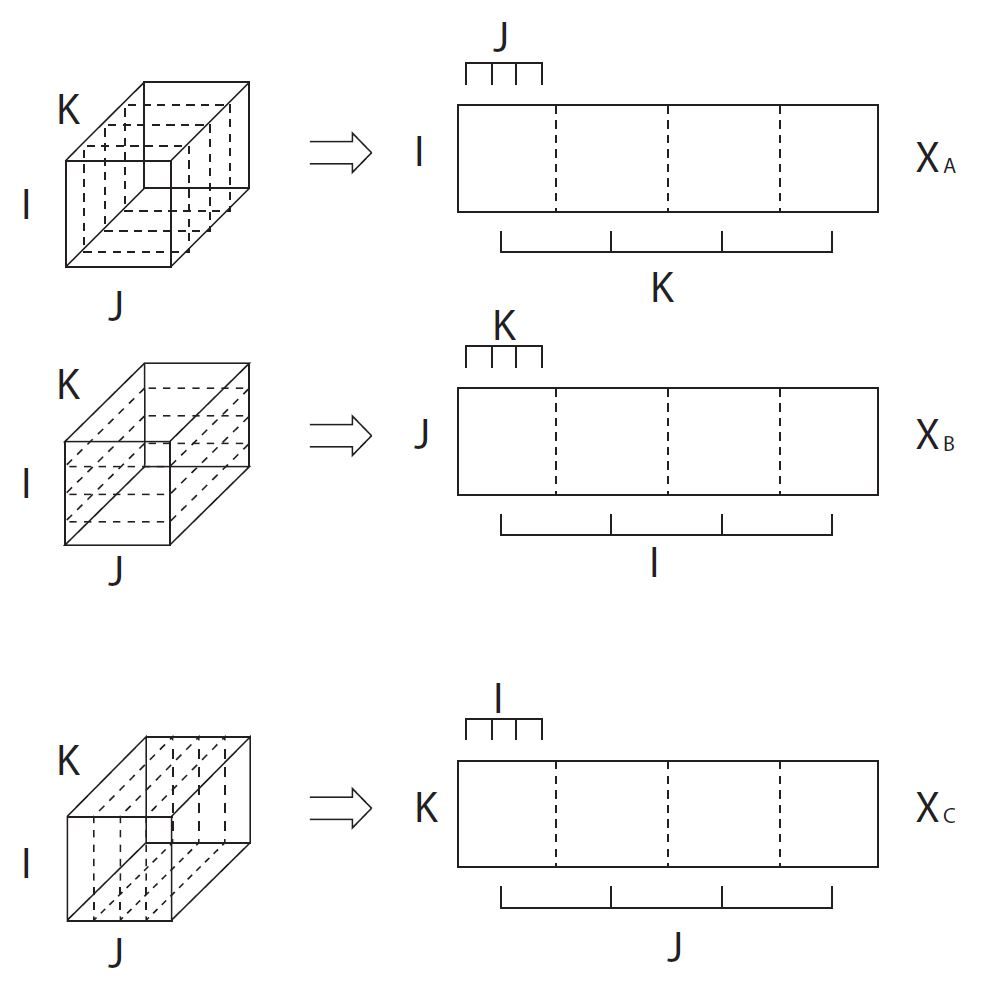
\includegraphics[width=0.7\textwidth]{matricization}
\caption{ Matricization of a three-way array into mode A matrix
$\vv{X}_A$, mode B matrix $\vv{X}_B$ and mode C matrix $\vv{X}_C$}
\label{fig-matricization}
\end{figure}
In some cases, particularly in most of the computational algorithms,
it is more convenient to represent the three-way array as a two dimensional
matrix by joining the slices in a specific way. This procedure is called
\emph{matricization} or \emph{unfolding} of the three dimensional array
and can be done in one of the three possible ways shown in
Fig.~\ref{fig-matricization} on the right. These matrices will be denoted in the code as
\code{Xa}, \code{Xb} and \code{Xc} respectively. To convert
a three-way array to one of these matrices the function \code{unfold()}
can be used, specifying the required mode (defaults to \code{mode="A"}).
To restore back a matricized array to a three dimensional array the
function \code{toArray()} is used. Let us consider as an example
\citep[][Section 2.6]{kiers2000towards} a $4 \times 3 \times 2$ array
consisting of the following two frontal slices:\\\\
$\begin{pmatrix}
1 & 2 & 0\\
0 & 1 & 0\\
1 & 0 & -1\\
-1 & 0 & 0
\end{pmatrix}$ and
$\begin{pmatrix}
0 & 1 & 0\\
1 & 0 & 0\\
1 & 2 & 0\\
0 & 0 & 1
\end{pmatrix}$

\begin{Schunk}
\begin{Sinput}
R> x <- c(1, 0, 1, -1, 2, 1, 0, 0, 0, 0, -1, 0, 0, 1, 1, 0, 1,
+      0, 2, 0, 0, 0, 0, 1)
R> X <- array(x, dim = c(4, 3, 2))
R> dimnames(X) <- list(1:4, 1:3, 1:2)
R> X
\end{Sinput}
\begin{Soutput}
, , 1

   1 2  3
1  1 2  0
2  0 1  0
3  1 0 -1
4 -1 0  0

, , 2

  1 2 3
1 0 1 0
2 1 0 0
3 1 2 0
4 0 0 1
\end{Soutput}
\begin{Sinput}
R> (Xa <- unfold(X))
\end{Sinput}
\begin{Soutput}
     [,1] [,2] [,3] [,4] [,5] [,6]
[1,]    1    2    0    0    1    0
[2,]    0    1    0    1    0    0
[3,]    1    0   -1    1    2    0
[4,]   -1    0    0    0    0    1
\end{Soutput}
\begin{Sinput}
R> (Xb <- unfold(X, mode = "B"))
\end{Sinput}
\begin{Soutput}
     [,1] [,2] [,3] [,4] [,5] [,6] [,7] [,8]
[1,]    1    0    0    1    1    1   -1    0
[2,]    2    1    1    0    0    2    0    0
[3,]    0    0    0    0   -1    0    0    1
\end{Soutput}
\begin{Sinput}
R> (Xc <- unfold(X, mode = "C"))
\end{Sinput}
\begin{Soutput}
     [,1] [,2] [,3] [,4] [,5] [,6] [,7] [,8] [,9] [,10] [,11] [,12]
[1,]    1    0    1   -1    2    1    0    0    0     0    -1     0
[2,]    0    1    1    0    1    0    2    0    0     0     0     1
\end{Soutput}
\end{Schunk}
These three forms of matricizations are related to each other by a
simple cyclic permutation of the modes, which is executed by
the function \code{permute()}. Another usage of the matricized
format is to read three-way arrays from and write to files.
\subsection{Model fitting interface}
\label{sec:interface}
The modeling interface of the \pkg{rrcov3way} consists of two main
functions, \code{Parafac()} and \code{Tucker3()} for estimating
the corresponding models. These functions take as an input a three-dimensional
data array and return an \code{S3} object \code{parafac} or \code{tucker3}
respectively. These objects are basically lists containing the estimated
loadings matrices \code{A}, \code{B} and \code{C} (plus the core
array \code{GA} in case of Tucker3), different estimation options and
results, like the fit value and the number of iterations performed,
as well as diagnostic output like the residual distances and the outlier flags.
On these objects a number of standard \proglang(R)~functions can be applied: \code{print()},
\code{show()}, \code{summary()}, \code{plot()} as well as a number of
postprocessing functions which will be described in the next section.
Whether to perform robust analysis is controlled by  the parameter
\code{robust=FALSE} (default) or \code{robust=TRUE}. Similarly, whether
to take into account the closeness of the data (compositional or not) is
controlled by the parameter \code{coda.transform="none"} or \code{coda.transform="ilr"}.
Of course this parameter could have been also logical like \code{robust},
but in this way we left the door open for implementing other transformations for
compositional data like the \emph{pivot coordinates} or \emph{weighted pivot coordinates}
\citep[see][]{filzmoser-book:2018}.
\subsubsection{Initialization of the algorithms}
For starting the ALS estimation it is necessary to provide
initial values of the loading matrices. Good starting values
could potentially  speed up the algorithm and ensure that the
global minimum  is found. By default the initial values are based on
an approximate solution obtained from the generalized
singular value decomposition. Alternatively the user
can select random start matrices by setting \code{stat="random"} or
provide a list of three matrices, to be used as starting values.\\\\
For stopping the iterations the  relative  change in fit between
two iterations is used, the algorithm stops if it is
below a certain value given by the parameter \code{conv}.
By default \code{conv=1e-6}.
\subsubsection{Constrained estimation for PARAFAC}
Sometimes it is necessary to constrain the PARAFAC solution
in order to improve the interpretability or for other reasons.
In psychometrics orthogonality constraints are often used
as a means of overcoming  problems with unstable solutions. In
chemometrics the preferred constraint is nonnegativity of
the solution producing nonnegative loadings. A general method
to find the least squares  loading  vector given  a nonnegativity  constraint
has been proposed by \citet{lawson:nnls} which is implemented
in the \proglang{R}~package \pkg{nnls}. Constraints are requested from
the \code{Parafac()} function using the parameter \code{const}.
The default is \code{const="none"} for no constraints. Orthogonality
constraints for all modes are requested by \code{const="orth"},
nonnegativity constraints by \code{const="nonneg"} and
\code{const="zerocor"} means zero correlations constraints.
Examples for using nonnegativity constraints in PARAFAC
can be found in Section~\ref{sec:ex-amino}.
\subsubsection{Parameters for robust estimation}
Selecting \code{robust=TRUE} in the call of the modeling
function (\code{Parafac()} or \code{Tucker3()}), robust
estimation will be performed for which several more
parameters can be selected.\\\\
First of all the level of robustness,
the so called breakdown point can be set between 0.5 (maximal robustness) and 0 (no robustness).
This is done through the parameter \code{alpha} which is passed to the function
\code{PcaHubert()}. The default value is \code{alpha=0.75} which gives
high robustness of 25\% and acceptable efficiency. It can be changed to a value in the range from
\code{alpha=0.5} for maximal robustness to \code{alpha=1} for no robustness.\\\\
The next parameter related to robustness is the number of components $k$ to use in the robust PCA
carried out in the first step of the robust PARAFAC or Tucker3 algorithms. By default
\code{ncomp.rpca=0} which forces the algorithm to find $k$ such that $l_k/l_1
\ge 10^{-3}$ and $\sum_{j=1}^k l_j/\sum_{j=1}^r l_j \ge 0.8$, where $l_1, \ldots, l_r$
are the eigenvalues of the sample covariance matrix of the data.
Alternatively the number of principal components $k$ can be
specified by the user after inspecting the scree plot. Both \code{Parafac()} and
\code{Tucker3()} functions return a PCA object \code{pcaobj} which can be used to
visualize the scree plot as follows:
\begin{Schunk}
\begin{Sinput}
R> data("elind")
R> (o <- Parafac(elind, robust = TRUE, ncomp.rpca = 11))
\end{Sinput}
\begin{Soutput}
Call:
Parafac(X = elind, robust = TRUE, ncomp.rpca = 11)


PARAFAC analysis with  2  components.
Fit value: 243.5351 
Fit percentage: 85.12 %
Robust
\end{Soutput}
\begin{Sinput}
R> rrcov::screeplot(o$pcaobj, main = "Screeplot: elind data")
R> o1 <- Parafac(elind, robust = TRUE)
R> cat("\n Selected number of components: ", o1$pcaobj$k, "\n")
\end{Sinput}
\begin{Soutput}
 Selected number of components:  4 
\end{Soutput}
\end{Schunk}
\begin{figure}[H]
\centering
\includegraphics[width=0.7\textwidth]{images/rrcov3way-robust-pca}\\
\caption{Selecting the number of components for robust PCA: The screeplot.}
\label{fig-robust-pca}
\end{figure}
The screen plot suggests 4 components, but this is also the number of components
which will be selected by the default method described above.
For more details on robust PCA in \proglang{R} see \citep{todorov-oof}.\\\\
Another parameter related to robust estimations is \code{robiter} which
specifyies the maximal number of ALS iterations necessary to achieve a robust fit.
By default \code{robiter=100} which in most of the cases is sufficient.\\\\
The last robustness parameter is \code{crit} which specifies the quantile
for identifying outliers, for example in the outlier map plot
shown in Fig.~\ref{fig-girls-ddplot}.
\subsection{Preprocessing}
\label{sec:preprocessing}
In three-way analysis, in the same way as in multivariate analysis it
is important to prepare the data before starting the actual analysis.
Often this preprocessing is a complex procedure, specific for the
application domain \citep[see for example][]{Engelen:2007}. The most
general preprocessing functions are removing the possible offset (centering)
and bringing the variables to the same scale (scaling or normalizing). While
in multivariate analysis these procedures are straightforward, in
three-way analysis we have more options (modes) of doing this. The most
standard preprocessing procedure is to center across the first (A) mode
and to normalize within the second (B) mode. This will (in most of the cases)
eliminate differences in levels and scales which are not natural to the data.
It is important to note that the multivariate methods,
including PARAFAC and Tucker3, require ratio-scale  data.
Ratio scale data are represented by proportional values and the lack
of the measured property is embodied by the zero. Usually data at hand are
interval scaled and the centering procedure will turn them into ratio-scaled.
If data are not approximately ratio-scaled, centering is mandatory.
On the other hand, scaling is related to the estimation procedure
and is intended to make the data compatible with the least squares.\\\\
Centering across a mode (by default mode A is selected) is performed by
first matricizing the array into the selected mode and then subtracting
a column measure of location from the columns of the matrix (same as in two way analysis).
If the selected location is the arithmetic mean the centering for mode A is done as follows :
\[z_{ijk}=x_{ijk}-\bar x_{.jk}=x_{ijk} - \frac{1}{I}\sum \limits_{i=1}^I x_{ijk}
\]
Since only a single mode is affected, this is usually called single centering.
In a similar way centering is applied to any other mode. In the package \pkg{rrcov3way}
centering is done by the function \code{do3Scale()}, setting the parameter \code{center=TRUE}.
We try this on the OECD data set (we could skip \code{center.mode="A"}
since this is the default). Setting \code{center=TRUE} will by default subtract the
arithmetic mean, but it is possible to specify any suitable function,
for example \code{center=median} will subtract the median.
\begin{Schunk}
\begin{Sinput}
R> elind.cA <- do3Scale(elind, center = TRUE, center.mode = "A")
R> round(colMeans(elind.cA[, , 1]), 10)
\end{Sinput}
\begin{Soutput}
INFO RADI TELE STRU ELET COMP 
   0    0    0    0    0    0 
\end{Soutput}
\end{Schunk}
If it is necessary to center across several modes, this is done sequentially,
providing the result of one operation to the next. The first centering
(say,  across  mode A) will not be destroyed.
\begin{Schunk}
\begin{Sinput}
R> elind.cAB <- do3Scale(elind.cA, center = TRUE, center.mode = "B")
R> round(colMeans(elind.cAB[, , 1]), 10)
\end{Sinput}
\begin{Soutput}
INFO RADI TELE STRU ELET COMP 
   0    0    0    0    0    0 
\end{Soutput}
\end{Schunk}
Differently from centering, it is not appropriate to scale the unfolded
array column-wise, but rather whole submatrices of the array should be scaled.
Mathematically scaling within mode B can be described as follows:
\[
 z_{ijk}=\frac{x_{ijk}}{\sqrt{\left( \sum \limits_{i=1}^I \sum \limits_{k=1}^K x_{ijk^2} \right)} }
\]
The scaling is also done by the function \code{do3Scale()} setting \code{scale=TRUE}.
The default mode is B. If required to scale not by the sum of squares but by the
standard deviation as usually done in profile analysis \citep[see][]{kroonenberg:2009},
we simply set the scale parameter to the function: \code{scale=sd}.
\begin{Schunk}
\begin{Sinput}
R> elind.cAsB <- do3Scale(elind, center = TRUE, scale = TRUE)
\end{Sinput}
\end{Schunk}
If robust scaling is required we could use some robust alternative of the scale function, like $MAD$ or $Q_n$.
\begin{Schunk}
\begin{Sinput}
R> elind.cAsB <- do3Scale(elind, center = TRUE, scale = mad)
\end{Sinput}
\end{Schunk}
Let us consider the following very simple simulated example \citep{bro:1998-2008}, where,
with the matrices $A=B=C= (1, 2, 3, 4 )^\top$ a PARAFAC model $X=A (B \otimes C)^\top$ is constructed.
The estimated model with one component has 100\% fit and it obtains the same fit if the data are
scaled across the first mode. If we center by subtracting the
grand average, the fit drops dramatically.
\begin{Schunk}
\begin{Sinput}
R> A <- B <- C <- matrix(c(1, 2, 3, 4)) + 10
R> X0 <- A %*% t(krp(C, B))
R> X <- toArray(X0, 4, 4, 4)
R> Parafac(X, ncomp = 1)$fp
\end{Sinput}
\begin{Soutput}
[1] 100
\end{Soutput}
\begin{Sinput}
R> Parafac(do3Scale(X, center = TRUE), ncomp = 1)$fp
\end{Sinput}
\begin{Soutput}
[1] 100
\end{Soutput}
\begin{Sinput}
R> Parafac(X - mean(X), ncomp = 1)$fp
\end{Sinput}
\begin{Soutput}
[1] 50.11853
\end{Soutput}
\begin{Sinput}
R> Parafac(do3Scale(X, center = TRUE, scale = TRUE), ncomp = 1)$fp
\end{Sinput}
\begin{Soutput}
[1] 100
\end{Soutput}
\end{Schunk}
Instead of doing the centering and scaling in advance, it is possible to
instruct the \code{Parafac()} and \code{Tucker3()} functions to do this by
setting the parameters \code{center=TRUE} and/or \code{scale=TRUE}.
\subsection{Postprocessing}
\label{sec:postprocessing}
Once the parameters are estimated and the model is built,
different procedures can be applied on the solution in order
to facilitate the interpretation. These can be different
transformations and rotations, rescaling of components and/or core array,
reflecting the sign or reordering the components.
\paragraph{Renormalization.} Once the solution is obtained, it could be necessary to
scale the components in order to make them comparable across modes or to
facilitate plotting. \cite{kroonenberg:2008} considers three ways of
adjusting the components for subsequent analysis and visualization and
the most basic of them is the \emph{renormalization}, i.e., bringing the
components to a unit length, i.e., $\sum a_{ip}^2 = 1$ for each component
$p=1, \ldots, P$. The components returned by the Tucker3 algorithm
implemented in the function \code{Tucker3()} are already normalized,
but it is possible that one wants the core array to be normalized.
The components returned by the PARAFAC algorithm are by default
not normalized. It is important to note, that it is necessary to
compensate the scaling of components by the inverse scaling of
the core array or other components. Renormalization is done by the
S3 method \code{do3Scale()} for Tucker3 or PARAFAC respectively.
With the following script the core array of the Tucker3 model
will be normalized to unit row sums and the compensation will
be absorbed by the A mode (default). With \code{renorm="B"} we
can choose another mode to absorb the compensation.
\begin{Schunk}
\begin{Sinput}
R> t3 <- Tucker3(elind, 3, 2, 2)
R> t3.norm <- do3Scale(t3, renorm.mode = "A")
R> rowSums(t3.norm$GA ^ 2)
\end{Sinput}
\begin{Soutput}
F1 F2 F3 
 1  1  1 
\end{Soutput}
\end{Schunk}
Similarly, in PARAFAC with for example \code{renorm="A"} (default) we
choose to renormalize the components of the modes B and C to unit length
while the components of mode A will absorb the compensation.
\begin{Schunk}
\begin{Sinput}
R> cp <- Parafac(elind, ncomp = 3)
R> cp.norm <- do3Scale(cp, renorm.mode = "A")
R> colSums(cp.norm$B ^ 2)
\end{Sinput}
\begin{Soutput}
F1 F2 F3 
 1  1  1 
\end{Soutput}
\begin{Sinput}
R> colSums(cp.norm$C ^ 2)
\end{Sinput}
\begin{Soutput}
F1 F2 F3 
 1  1  1 
\end{Soutput}
\end{Schunk}
\paragraph{Rotation.}
As already mentioned in the introduction, the decomposition provided by
the Tucker3 model is not unique. Any arbitrary nonsingular rotation of
all components simultaneously will retain the model representation
and thus will produce a new solution. \citet{Tucker:1966} showed that
postmultiplying $\vv{A}, \vv{B}$, and $\vv{C}$ by non singular matrices,
i.e., $\vv{L}, \vv{M}$, and $\vv{N}$, can always be compensated for by
applying the inverse of these matrices to the core array. It can be
verified that
\begin{equation}
\vv{X}_A = \vv{A}\vv{G}_A(\vv{C} \otimes \vv{B})^\top + \vv{E}_A= \tilde{\vv{A}}\tilde{\vv{G}}_A(\tilde{\vv{C}} \otimes \tilde{\vv{B}})^\top + \vv{E}_A
\end{equation}
with $\tilde{\vv{A}}=\vv{AL}^{-1}$, $\tilde{\vv{B}}=\vv{BM}^{-1}$, $\tilde{\vv{C}}=\vv{CN}^{-1}$ and $\tilde{\vv{G}}_A=\vv{L}\mathbf{G}_A (\vv{N} \otimes \vv{M})$.
This rotational freedom of
the Tucker3 model can be exploited to obtain a simplified, easier
to interpret form of the core array. Since such rotation can distort
the simplicity of the component matrices, a trade-off can be searched for,
as proposed by \citet{kiers1998orthomax}. This is a general procedure
for joint rotation of the core array and the component matrices,
allowing any combination of relative weights to be attached to
the simplicity of core versus the simplicity of the component matrices.\\\\
In \pkg{rrcov3way} this method is implemented in the function \code{do3rotation()}
which transforms a Tucker3 solution into a simpler one using the provided
as parameters relative weights. By default the rotation is done on all
modes: \code{rotate=c("A", "B", "C")}.
To illustrate the use of this function,
the OECD data \code{elind} will be used. In the following example the
Tucker3 solution with 3x2x2 components will be simplified by rotating all three component
matrices using equal relative weights $w_A=w_B=w_C=3$. The function will
update the solution \code{t3} with the rotated core \code{t3$GA} and the component matrices
\code{A}, \code{B} and \code{C}. The varimax values will be returned (in \code{vvalue})
as well as the rotation matrices \code{S}, \code{T} and \code{U}.
\begin{Schunk}
\begin{Sinput}
R> data("elind")
R> t3 <- Tucker3(elind, 3, 2, 2)
R> xout <- do3Rotate(t3, c(3, 3, 3), rotate = c("A", "B", "C"))
R> xout$vvalue
\end{Sinput}
\end{Schunk}

\begin{Schunk}
\begin{Soutput}
      GA        A        B        C 
3.136374 5.888002 2.543755 1.378694 
\end{Soutput}
\end{Schunk}

With relative weights all equal to 0, $w_A=w_B=w_C=0$,
maximal simplicity of the core array is achieved. On the other hand,
all weights equal to infinity yield maximal simplicity of the component matrices.
By choosing appropriate combination of the weights, reasonable simplicity of
both the core array and the component matrices can be obtained. The following
Table~\ref{tab:varimax} shows the varimax values for the core array and
the component matrices for different joint varimax rotations (given by different
relative weights) to the Tucker3 solution with 3x2x2 components of the OECD data.
% latex table generated in R 4.5.0 by xtable 1.8-4 package
% Sat Jul  5 14:53:47 2025
\begin{table}[H]
\centering
\begin{tabular}{rrrrrrrr}
  \hline
 & w(A) & w(B) & w(C) & Core & A & B & C \\ 
  \hline
1 &  &  &  & 6.87 & 4.48 & 1.39 & 0.74 \\ 
  2 & 0.00 & 0.00 & 0.00 & 6.88 & 4.44 & 1.42 & 0.72 \\ 
  3 & 0.50 & 0.50 & 0.50 & 6.70 & 4.86 & 1.69 & 0.80 \\ 
  4 & 1.00 & 1.00 & 1.00 & 6.15 & 5.18 & 2.01 & 0.89 \\ 
  5 & 2.50 & 2.50 & 2.50 & 3.64 & 5.82 & 2.51 & 1.30 \\ 
  6 & 3.00 & 3.00 & 3.00 & 3.14 & 5.89 & 2.54 & 1.38 \\ 
  7 & 3.50 & 3.50 & 3.50 & 2.81 & 5.93 & 2.56 & 1.43 \\ 
  8 & 4.00 & 4.00 & 4.00 & 2.60 & 5.95 & 2.56 & 1.46 \\ 
  9 & 5.00 & 5.00 & 5.00 & 2.33 & 5.97 & 2.57 & 1.49 \\ 
  10 & 10.00 & 10.00 & 10.00 & 1.93 & 5.99 & 2.57 & 1.52 \\ 
  11 & Inf & Inf & Inf & 1.65 & 6.00 & 2.57 & 1.53 \\ 
   \hline
\end{tabular}
\caption{Varimax values for
the core array and the component matrices for different joint
varimax rotations to the Tucker3 solution with 3x2x2 components
of the OECD data} 
\label{tab:varimax}
\end{table}From this table we can see that the solution with all relative weights equal to 3 is
the best compromise between simplicity of core array and component matrices.
The next four tables show the unrotated and rotated with relative weights
(3, 3, 3) solutions and allow to observe to what extent the
interpretability of the model was improved.
% latex table generated in R 4.5.0 by xtable 1.8-4 package
% Sat Jul  5 14:53:47 2025
\begin{table}[H]
\centering
\begin{tabular}{rrrrrrr}
  \hline
 & F1 & F2 & F3 & F1 & F2 & F3 \\ 
  \hline
CA & -0.16 & -0.05 & 0.06 & 0.17 & -0.02 & 0.02 \\ 
  US & -0.16 & -0.06 & 0.07 & 0.18 & -0.03 & 0.01 \\ 
  JP & -0.21 & 0.33 & -0.11 & 0.02 & 0.18 & 0.36 \\ 
  AS & -0.18 & -0.17 & 0.02 & 0.23 & 0.02 & -0.09 \\ 
  NZ & -0.22 & -0.23 & -0.11 & 0.27 & 0.14 & -0.15 \\ 
  BL & -0.23 & 0.23 & -0.04 & 0.10 & 0.12 & 0.29 \\ 
  DA & -0.26 & -0.02 & 0.13 & 0.27 & -0.06 & 0.10 \\ 
  FR & -0.19 & -0.15 & 0.07 & 0.25 & -0.03 & -0.05 \\ 
  RF & -0.22 & -0.01 & 0.05 & 0.21 & 0.01 & 0.08 \\ 
  GR & -0.24 & -0.32 & 0.13 & 0.37 & -0.08 & -0.17 \\ 
  IR & -0.11 & -0.05 & 0.00 & 0.11 & 0.02 & -0.00 \\ 
  IT & -0.17 & -0.06 & 0.07 & 0.19 & -0.02 & 0.02 \\ 
  PB & -0.20 & -0.02 & -0.04 & 0.18 & 0.09 & 0.05 \\ 
  RU & -0.15 & -0.08 & 0.09 & 0.19 & -0.05 & 0.00 \\ 
  AU & -0.25 & 0.26 & 0.03 & 0.12 & 0.06 & 0.34 \\ 
  FI & -0.27 & 0.33 & -0.14 & 0.07 & 0.24 & 0.38 \\ 
  NO & -0.17 & -0.17 & 0.04 & 0.23 & -0.01 & -0.08 \\ 
  PO & -0.20 & 0.55 & 0.37 & 0.03 & -0.26 & 0.64 \\ 
  SP & -0.17 & -0.07 & 0.06 & 0.19 & -0.01 & 0.01 \\ 
  SV & -0.20 & -0.12 & 0.07 & 0.24 & -0.03 & -0.02 \\ 
  CH & -0.23 & -0.29 & 0.15 & 0.36 & -0.10 & -0.15 \\ 
  TU & -0.26 & -0.00 & -0.84 & 0.04 & 0.88 & -0.05 \\ 
  YU & -0.26 & -0.04 & 0.13 & 0.27 & -0.06 & 0.09 \\ 
   \hline
\end{tabular}
\caption{Component matrix A from the unrotated and
    rotated solution with relative weights (3, 3, 3)} 
\label{tab:varimax-A}
\end{table}
% latex table generated in R 4.5.0 by xtable 1.8-4 package
% Sat Jul  5 14:53:47 2025
\begin{table}[H]
\centering
\begin{tabular}{rrrrr}
  \hline
 & F1 & F2 & F1 & F2 \\ 
  \hline
INFO & -0.26 & 0.09 & 0.02 & 0.28 \\ 
  RADI & -0.42 & -0.86 & 0.96 & 0.03 \\ 
  TELE & -0.46 & 0.26 & -0.05 & 0.53 \\ 
  STRU & -0.59 & 0.40 & -0.12 & 0.70 \\ 
  ELET & -0.34 & 0.07 & 0.08 & 0.34 \\ 
  COMP & -0.28 & -0.14 & 0.25 & 0.19 \\ 
   \hline
\end{tabular}
\caption{Component matrix B from the unrotated and
    rotated solution with relative weights (3, 3, 3)} 
\label{tab:varimax-B}
\end{table}
% latex table generated in R 4.5.0 by xtable 1.8-4 package
% Sat Jul  5 14:53:47 2025
\begin{table}[H]
\centering
\begin{tabular}{rrrrr}
  \hline
 & F1 & F2 & F1 & F2 \\ 
  \hline
78 & -0.33 & -0.75 & 0.81 & 0.09 \\ 
  79 & -0.36 & -0.37 & 0.46 & 0.23 \\ 
  80 & -0.34 & -0.14 & 0.24 & 0.28 \\ 
  82 & -0.38 & 0.28 & -0.15 & 0.45 \\ 
  83 & -0.40 & 0.25 & -0.11 & 0.46 \\ 
  84 & -0.41 & 0.28 & -0.14 & 0.48 \\ 
  85 & -0.41 & 0.27 & -0.13 & 0.47 \\ 
   \hline
\end{tabular}
\caption{Component matrix C from the unrotated and
    rotated solution with relative weights (3, 3, 3)} 
\label{tab:varimax-C}
\end{table}
% latex table generated in R 4.5.0 by xtable 1.8-4 package
% Sat Jul  5 14:53:47 2025
\begin{table}[H]
\centering
\begin{tabular}{rrrrr}
  \hline
 & F1 & F2 & F3 & F4 \\ 
  \hline
F1 & -32.69 & 0.27 & -0.46 & -1.70 \\ 
  F2 & 0.19 & 12.48 & -1.03 & -1.45 \\ 
  F3 & 0.29 & -0.72 & -0.77 & -5.55 \\ 
  X &  &  &  &  \\ 
  F1.1 & 3.07 & 8.91 & 6.06 & 27.18 \\ 
  F2.1 & 6.74 & 0.67 & 3.01 & 7.40 \\ 
  F3.1 & 2.88 & 2.03 & 15.18 & 6.81 \\ 
   \hline
\end{tabular}
\caption{Core array from the unrotated and rotated
    solution with relative weights (3, 3, 3)} 
\label{tab:varimax-core}
\end{table}
\paragraph {Reflection (or sign reversal).} The sign reversal
does not change the model (PARAFAC or Tucker3) as long as
it is done consistently \citep[see][p.200]{smilde:2004}. The
flip of the sign (multiplying by -1) in PARAFAC has to be done
simultaneously on two modes (A and B or A and C or B and C), while
in Tucker3 this is more complicated because of the presence
of the core array. The sign reversal will cause a mirroring
of the scatter plot (see~\ref{sec:visual}). In \pkg{rrcov3way} reflection
is done either by one of the methods \code{reflect()} or \code{do3Postprocess()}.
In the following example the sign of the second component of mode
A of a PARAFAC model will be flipped (and this change will be absorbed by mode B).
\begin{Schunk}
\begin{Sinput}
R> res <- Parafac(elind)
R> head(res$A)
\end{Sinput}
\begin{Soutput}
         F1         F2
CA 5.278714 -0.7455495
US 5.405461 -0.7422575
JP 6.633099  0.3431131
AS 6.156730 -1.2995336
NZ 7.683093 -1.7930409
BL 7.568537 -0.1430425
\end{Soutput}
\begin{Sinput}
R> head(res$B)
\end{Sinput}
\begin{Soutput}
             F1          F2
INFO -0.2481020  0.03797682
RADI -0.7860668 -2.72317282
TELE -0.3548324  0.68392392
STRU -0.4097308  1.18703648
ELET -0.3352797 -0.01079269
COMP -0.3627819 -0.67860306
\end{Soutput}
\begin{Sinput}
R> res1 <- do3Postprocess(res, reflectA = c(1, -1))
R> head(res1$A)
\end{Sinput}
\begin{Soutput}
         F1         F2
CA 5.278714  0.7455495
US 5.405461  0.7422575
JP 6.633099 -0.3431131
AS 6.156730  1.2995336
NZ 7.683093  1.7930409
BL 7.568537  0.1430425
\end{Soutput}
\begin{Sinput}
R> head(res1$B)
\end{Sinput}
\begin{Soutput}
             F1          F2
INFO -0.2481020 -0.03797682
RADI -0.7860668  2.72317282
TELE -0.3548324 -0.68392392
STRU -0.4097308 -1.18703648
ELET -0.3352797  0.01079269
COMP -0.3627819  0.67860306
\end{Soutput}
\end{Schunk}
\paragraph{Reordering the components.} Similarly as the sign reversal,
reordering of the components will not change the model if done consistently
(for all modes simultaneously in PARAFAC and for the selected mode
and the core array in Tucker3). In \pkg{rrcov3way} reordering
is done by one of the methods \code{reorder()} or \code{do3Postprocess()}.
The parameter \code{order} can be either a vector containing the new order
of the components or a logical \code{TRUE}. In the latter case the
components will be arranged in decreasing order of the component
standardized weights (explained variability).
\subsection{Visual tools for three-way analysis}
\label{sec:visual}
The results from a three-way analysis can be presented in
several different ways \citep[see][]{kroonenberg:2009}, the first one
being tables of the coefficients or loadings for each mode, either rotated or not.
While it is important to inspect the numerical output of the
methods for analysis of three-way data (the component matrices
and the core array) in order to properly interpret the results,
it can be of great help to use different visual representations of these outcomes.
The most typical plots are:
\bi
\item Distance-distance plot for presenting robust models and identifying outliers,
\item Pair-wise graphs of the components for each mode separately,
\item All-components plots which will show all components of a single mode using the levels of the mode as X-axis,
\item Per-component plot, showing a single component on
all modes simultaneously in the same plot.
\ei
As we will see further, although all these plots can be applied
to both PARAFAC and Tucker3 models, some of them (e.g., the
per-component plots) are more suitable for the results of
PARAFAC, while others are more suitable for Tucker3 (e.g., the joint biplots).\\\\
One of the features of the package \pkg{rrcov3way} which is not
to be found in the other \proglang{R} packages for three-way analysis,
is the availability of a variety of plotting procedures. These
procedures are flexible enough to give the user the possibility
to design the graphs according to the needs and the data at hand
but at the same time provide suitable default parameters which
facilitate their use. These procedures are mainly based on
\citet{kiers2000some} and \citet{kroonenberg:2008} and the reader
is referred to these publications for more details. \\\\
To illustrate the plotting procedures in the package the data set
\code{girls} \citep{kroonenberg:2008} will be used. It is available
in the package and we start by loading it.
\begin{Schunk}
\begin{Sinput}
R> data("girls")
R> dim(girls)
\end{Sinput}
\begin{Soutput}
[1] 30  8 12
\end{Soutput}
\begin{Sinput}
R> head(girls[, , 1])
\end{Sinput}
\begin{Soutput}
  weight length crrump head chest arm calf pelvis
1   1456   1025    602  486   520 157  205    170
2   1426    998    572  501   520 150  215    169
3   1335    961    560  494   495 145  214    158
4   1607   1006    595  497   560 178  218    172
5   1684   1012    584  490   553 165  220    158
6   1374   1012    580  492   525 158  202    167
\end{Soutput}
\begin{Sinput}
R> sum(girls ^ 2)
\end{Sinput}
\begin{Soutput}
[1] 5013808343
\end{Soutput}
\end{Schunk}
The data are from a French auxiological study in the years 1953---1975,
\citep{sempe:1987} with the goal to
get insight into the physical growth patterns of children from ages
four to fifteen. Thirty girls were selected and they were measured
yearly between the ages 4 and 15 on the following eight variables:
\bi
\item 	Weight,
\item 	Length,
\item	Crown-rump length,
\item	Head circumference,
\item	Chest circumference,
\item	Arm,
\item	Calf,
\item	Pelvis.
\ei
The data are stored as a three-way array of size
30(girls) $\times$ 8(variables)  $\times$ 12(years). The data are
preprocessed by centering across mode A (the 30 girls), and by
normalizing each of the variables (i.e., across girls and years)
such that for each variable the sum of squares is unity. We do
the centering and normalization with the function \code{do3Scale()}, setting
\code{only.data=FALSE} in order to obtains also the center that was removed,
i.e., the profile of the ``average girl''. This average profile will be used
to plot in Fig.~\ref{fig-average-girl} the average growth curves.
To equalize the range of the variables,
several variables were divided by 10 (in the legend of the plot these
variables are marked by an asterisk.
\begin{Schunk}
\begin{Sinput}
R> X <- do3Scale(girls, center = TRUE, scale = TRUE, only.data = FALSE)
R> center <- X$center
R> X <- X$x
R> average.girl <- as.data.frame(matrix(center, ncol = 8, byrow = TRUE))
R> dimnames(average.girl) <- list(dimnames(X)[[3]], dimnames(X)[[2]])
R> average.girl$weight <- average.girl$weight / 10
R> average.girl$length <- average.girl$length / 10
R> average.girl$crrump <- average.girl$crrump / 10
R> sum(X ^ 2)
\end{Sinput}
\begin{Soutput}
[1] 8
\end{Soutput}
\end{Schunk}
\begin{Schunk}
\begin{Sinput}
R> p <- ncol(average.girl)
R> plot(rownames(average.girl), average.girl[,1],
+      ylim = c(50, 1200),
+      type = "n", xlab = "Age", ylab = "")
R> for(i in 1: p)
+  {
+      lines(rownames(average.girl), average.girl[, i], lty = i, col = i)
+      points(rownames(average.girl), average.girl[, i], pch = i, col = i)
+  }
R> legend <- colnames(average.girl)
R> legend[1] <- paste0(legend[1], "*")
R> legend[2] <- paste0(legend[3], "*")
R> legend[3] <- paste0(legend[4], "*")
R> legend("topleft", legend = legend, col = 1:p, lty = 1:p, pch = 1:p)
\end{Sinput}
\end{Schunk}
\begin{figure}[H]
\centering
\includegraphics{images/rrcov3way-girls-average-plot}\\
\caption{Average growth curves for the girls data set. The variables
with an asterisk were divided by 10 to make the ranges similar}
\label{fig-average-girl}
\end{figure}
To the preprocessed data will be applied Tucker3 analysis
with $P=3, Q=3$ and $R=2$ components and PARAFAC analysis with $F=3$ components,
as it was done in \citet{kroonenberg:2008}.
\begin{Schunk}
\begin{Sinput}
R> (t3 <- Tucker3(X, 3, 3, 2))
\end{Sinput}
\begin{Soutput}
Call:
Tucker3(X = X, P = 3, Q = 3, R = 2)


Tucker3 analysis with  3 x 3 x 2  components.
Fit value: 1.833182 
Fit percentage: 77.09 %
\end{Soutput}
\begin{Sinput}
R> (cp <- Parafac(X, ncomp = 3))
\end{Sinput}
\begin{Soutput}
Call:
Parafac(X = X, ncomp = 3)


PARAFAC analysis with  3  components.
Fit value: 1.808497 
Fit percentage: 77.39 %
\end{Soutput}
\end{Schunk}
Both models obtain a fit of 77.4\%. We execute also the robust Tucker3 procedure
by setting the argument \code{robust=TRUE}. For the underlying robust principal
components for both Tucker3 and PARAFAC, we select the number of components
to be \code{ncomp.rpca=3}, as suggested by the unfolded data array.
In this case the fit becomes 81\% for the robust Tucker and 82\% for
the robust PARAFAC models.
\begin{Schunk}
\begin{Sinput}
R> (t3r <- Tucker3(X, 3, 3, 2, robust = TRUE, ncomp.rpca = 3))
\end{Sinput}
\begin{Soutput}
Call:
Tucker3(X = X, P = 3, Q = 3, R = 2, robust = TRUE, ncomp.rpca = 3)


Tucker3 analysis with  3 x 3 x 2  components.
Fit value: 1.497163 
Fit percentage: 81.29 %
Robust
\end{Soutput}
\begin{Sinput}
R> (cpr <- Parafac(X, ncomp = 3, robust = TRUE, ncomp.rpca = 3))
\end{Sinput}
\begin{Soutput}
Call:
Parafac(X = X, ncomp = 3, robust = TRUE, ncomp.rpca = 3)


PARAFAC analysis with  3  components.
Fit value: 1.377797 
Fit percentage: 82.78 %
Robust
\end{Soutput}
\end{Schunk}
\paragraph{Distance-Distance plot.} In the context of PCA \cite{hubert-ROBPCA:2005}
defined a \emph{diagnostic plot} or \emph{outlier map} which
helps to distinguish between regular observations and
different types of outliers. Similarly as in robust regression \cite[see][]{Rousseeuw-van-Zomeren}
each observation is characterized by two distances: the residual distance (RD) defined in Equation~\ref{eq:rdist}
and the score distance (SD). The score distance of an observation $\vv{X}_i$
is the robust version of the Mahalanobis distance of the score $\vv{a}_i$
to the center of the score matrix $\vv{A}$:
\begin{equation}
\label{sdist}
\mbox{SD}_i=\sqrt{(\vv{a}_i - \vv{m})^\top \vv{S}^{-1}(\vv{a}_i - \vv{m})} ,
\end{equation}
where $\vv{m}$ and $\vv{S}$ are taken as the robust minimum
covariance determinant (MCD) estimates of the center and
covariance matrix of the scores respectively.
The diagnostic plot is constructed by plotting
the score distances on the horizontal axis, the residual
distances on the vertical axis and drawing two cutoff lines
which will help to classify the observations. The cutoff value on the
horizontal axis (for the score distances) is taken as the 97.5\% quantile of
$\chi^2_F$ distribution with $F$ degrees of freedom, i.e., $c_{horizontal}=\sqrt{\chi^2_{0.975, F}}$,
assuming that the scores are approximately normally distributed which gives
$\chi^2$-distributed squared score distances. For the cutoff value on the
vertical axis (for the residual distances) the Wilson-Hilferty transformation for a $\chi^2$ distribution
is used (which assumes that the $\text{RD}_i$ to the power of 2/3 are approximately
normally distributed). The parameters $\mu$ and $\sigma$ of the
normal distribution can be robustly estimated by the univariate MCD of the
values $\text{RD}_i^{2/3}$ as $m$ and $s$, and the critical value can be taken as
$c_{vertical}=(m + sz_{0.975})^{3/2}$ where $z_{0.975}$ is
the the 97.5\% quantile of the standard normal distribution.
Using these cutoff values the observations can be classified into regular observations
(small RD$_i$ and small SD$_i$), residual outliers (large RD$_i$ and small SD$_i$),
bad leverage points (large RD$_i$ and large SD$_i$) and good leverage points
(small RD$_i$ and large SD$_i$). \\\\
Similarly, a classical diagnostic plot can be generated by computing
the distances as well as their cutoff values using the classical
estimates instead of the robust ones. This will allow to compare visually
the classical and robust PARAFAC and Tucker3 methods. Both the robust and
the classical plot can be used for visualizing compositional data.\\\\
The distance-distance plot is the default plot for both Tucker3 and PARAFAC objects.
Therefore we can call the plot function, simply passing the
corresponding object as a parameter. The most extreme outliers
are identified by their labels. It is possible to specify the
number of outliers to be identified as well as the labels which are to be used.
In Fig.~\ref{fig-girls-ddplot} are shown the classical (left) and the robust (right)
distance-distance plots for PARAFAC model with \code{ncomp=3} of the girls data.
In the classical plot no bad leverage points are identified, only the girl
with label 27 is identified as  a residual outlier and girl 3 is possibly a border
case. Girl 30 is shown as a good leverage point. The robust  plot confirms
the outlying position of the girls 27 and 3, also shows girl 26 as a border
case, but also identifies girl 30 as a bed leverage point. Two other girls
are flagged as good leverage points (14 and 18).
\begin{figure}[H]
\centering
\includegraphics[width=0.7\textwidth]{images/rrcov3way-girls-ddplot}
\caption{Classical and robust distance-distance plot for a three component PARAFAC model of the girls data set.}
\label{fig-girls-ddplot}
\end{figure}
\paragraph{Paired components plots} (or single mode plots)
are plots in which pairs of components in a single mode
are plotted against each other in a two dimensional scatter plots.
\citet{kroonenberg:2008} differentiates between normalized
and principal coordinates, the former being the coordinates
returned by the estimation procedure and the latter are scaled
by the square root of the explained variance and argues that the
principal coordinates are preferred since they make the differences
in explained variances less dramatic. \citet{kiers2000some} proposes
a generic procedure, equivalent to the principal coordinates,
which we follow here. To generate this plot we use the argument
\code{which="comp"} in the generic plot function. The default
mode is A (can be changed by setting the argument \code{mode},
e.g., \code{mode="B"} or  \code{mode="C"}) and the default components to
plot are the first two but any combination of components can be chosen by
the argument \code{choices}, e.g., \code{choices=c(2,3)}. In case of
\code{mode="B"} the ``variables'' will be plotted as arrows, with
initial point in the origin. If this is not desired, the arrows can be suppressed
by \code{arrows=FALSE}. The paired components plots for mode A are shown
in Fig.~\ref{fig-girls-paired} and those for mode B (with arrows) in
Fig.~\ref{fig-girls-paired-B}.
\begin{Schunk}
\begin{Sinput}
R> oldpar <- par(mfrow = c(1, 2))
R> plot(t3, which = "comp", choices = 1L:2L)
R> plot(t3, which = "comp", choices = c(1L, 3L))
R> par(oldpar)
\end{Sinput}
\end{Schunk}
\begin{figure}[H]
\centering
\includegraphics[width=0.7\textwidth]{images/rrcov3way-girls-paired}
\caption{Side-by-side paired components plots of mode A of the girls growth curves data.}
\label{fig-girls-paired}
\end{figure}
\begin{Schunk}
\begin{Sinput}
R> oldpar <- par(mfrow = c(1, 2))
R> plot(t3, which = "comp", choices = 1L:2L, mode = "B")
R> plot(t3, which = "comp", choices = c(1L,3L), mode = "B")
R> par(oldpar)
\end{Sinput}
\end{Schunk}
\begin{figure}[H]
\centering
\includegraphics[width=0.7\textwidth]{images/rrcov3way-girls-paired-B}
\caption{Side-by-side paired components plots of mode B of the girls
growth curves data. The variables are presented as arrows.}
\label{fig-girls-paired-B}
\end{figure}
These displays are available for both Tucker3 and PARAFAC models, and
work in exactly the same way---this follows from the fact that
it is sufficient to replace the core array in Tucker3 by the
identity in PARAFAC. However, it is necessary to note that in the case of
a PARAFAC model the components are orthonormalized in accordance with
the Kiers' procedure \citep{kiers2000some}.\\\\
If the data are compositional, the orthonormalization will not affect the results.\\\\
\paragraph{Per-component plot.} This plot presents a single component across all modes.
In some cases one is not interested in the relation between the
different subjects which can be presented in one mode but rather in the relation
of the components in the different modes. The per-component plot is
constructed by plotting the coefficients for all modes along a single line.
Although this plot could be used also for Tucker3, it is most
suitable for PARAFAC. To facilitate the presentation of the different modes
on a single plot the components should be either orthonormalized or
scaled to unit mean square. The per-component plot for the girls
growth curve data is shown in Fig.~\ref{fig-girls-percomp}.
\begin{Schunk}
\begin{Sinput}
R> cp <- Parafac(X, ncomp = 2)
R> cp <- do3Postprocess(cp, reflectA = -1, reflectC = -1)
R> plot(cp, which = "percomp")
\end{Sinput}
\end{Schunk}
\begin{figure}[H]
\centering
\includegraphics[width=0.7\textwidth]{images/rrcov3way-girls-percomp}
\caption{Per-component plot for the girls growth curves data from a PARAFAC analysis with 2 components.}
\label{fig-girls-percomp}
\end{figure}
It is important to note that the variable means were removed for each
time point which means that the girl with zero component on the girls mode
is the average girl and has average growth curves. All variables and all
years have positive coefficients. The differences in variable 'Length' are
more dramatic than the differences in 'Arm circumference'. The time points
present something like trajectory up to the 13th year the differences
grow and after that fall down again.
\paragraph{All components plots.} These plots are also single mode plots and
are useful in case when one of the modes has a natural ordering---points
in time or wavelengths of emission/excitation spectra (the latter is
almost a standard plot in chemometrics). The two components from the
age mode (mode C) of the Tucker3 model of the girls growth curves data are presented
in Fig.~\ref{fig-girls-allcomp}.
\begin{Schunk}
\begin{Sinput}
R> plot(t3, which="allcomp")
\end{Sinput}
\end{Schunk}
\begin{figure}[H]
\centering
\includegraphics[width=0.7\textwidth]{images/rrcov3way-girls-allcomp}
\caption{All components plot for the girls growth curves data with the age
on the horizontal axis (mode C) and the component scores on the vertical axis.}
\label{fig-girls-allcomp}
\end{figure}
The second example is from chemometrics
and returns an \emph{all component plot} of a
PARAFAC model with three components of a fluorescence spectroscopy
experiment (Fig.~\ref{fig-amino-allcomp}). The data set is \code{amino} containing 5 samples (mode A) of
emission-excitation data. In the plot is presented the excitation mode (C)
on 61 wavelengths from 240 to 300. More about this data set can be found
in Section~\ref{sec:ex-amino}.
\begin{Schunk}
\begin{Sinput}
R> data("amino")
R> amino.cp <- Parafac(amino, ncomp = 3, const = "nonneg")
R> plot(amino.cp, which = "allcomp",
+      xlab = "Wavelength", ylab = "Intensity", mode = "C",
+      points = FALSE, legend.position = NULL)
\end{Sinput}
\end{Schunk}
\begin{figure}
\centering
\includegraphics[width=0.7\textwidth]{images/rrcov3way-amino-allcomp}
\caption{All components plot for the Anderson data---plot of PARAFAC
components of the excitation mode (mode C).}
\label{fig-amino-allcomp}
\end{figure}

%%  \paragraph{Oblique components plots}
%5  \textcolor{red}{see \citet{kroonenberg:2008}, 11.4.4 on page 269 and \citet{kiers2000some}, 5.2 on page 160.}

\paragraph{Joint biplots} In (two-way) multivariate analysis the biplot introduced by
\cite{gabriel} in the context of principal component analysis, represents
both the observations and variables in the plane of (the first) two principal components
allowing the visualization of the magnitude and sign of each variable's contribution to these
principal components. Each observation (row of scores) is represented as a point in the biplot
and each variable is represented as an arrow. The arrows graphically indicate the proportion
of the original variance explained by the (first) two principal components and their direction
indicates the relative loadings on these components. The biplot is constructed by
SVD decomposition of a data matrix $\vv{Y}=\vv{U}\vv{\Lambda}\vv{V}^\top$ where $\vv{U}$
and $\vv{V}$ are the orthonormal matrices of the left and right singular vectors
and $\vv{\Lambda}$ is a diagonal matrix of the ordered singular values
(i.e., the square roots of the eigenvalues). From this decomposition  two matrices
$\vv{A}$ and $\vv{B}$ are obtained, which contain coordinates for plotting
the subjects and the variables on the same display.\\\\
In three-way analysis we have three modes and it is necessary to choose two
of them as \emph{display} modes and use the third one as a \emph{reference} mode.
For each slice of the core array (for each component of the reference mode)
can be constructed a joint biplot. The \emph{joint biplot axis} are given by
\begin{equation}
\label{eq:JB-axes-1}
\tilde{\vv{A}_r} = (I/J)^{0.25}\vv{A}\vv{U}_r\vv{\Lambda}_r^{\alpha}
\end{equation}
and
\begin{equation}
\label{eq:JB-axes-2}
\tilde{\vv{B}_r} = (J/I)^{0.25}\vv{B}\vv{V}_r\vv{\Lambda}_r^{1-\alpha}
\end{equation}
where $\vv{U}_r\vv{\Lambda}\vv{V}_r^\top$ is the singular value decomposition
of the $r$-th slice $\vv{G}_r$ of the core array $\vv{G}$. For all the details
of the construction of the joint biplot of Tucker3 model
see \cite{kroonenberg:2008}, p.273 and the references thereafter.\\\\
Let us now consider an example joint biplot using the Tucker3 model of the
girls' growth curves data. As a reference mode we choose the time mode
(see the components of the time mode depicted in the all-components plot in
Fig.~\ref{fig-girls-allcomp}). In the first component we can observe steady
increase up to the thirteenth year and then a decline in the last two years.
The straightforward interpretation of the first component would be the overall
variability, meaning that the differentiation between the girls increases
up to the thirteenth year and after that the difference decreases in the
last two years. The joint biplot of the girls and variables modes taking
the age mode as a reference one is constructed by the plot command using
the argument \code{which="jbplot"}. By default the third mode is selected
as a reference mode and again by default the slicing of the core array
is done by the first component.
The resulting plot is shown in Fig.~\ref{fig-girls-jointbiplot}.
The first component of the age mode is presented. The first striking feature
in the plot is that the variables fall into two main groups: length variables
and circumference (soft tissue) variables.
\begin{Schunk}
\begin{Sinput}
R> t3x <- do3Postprocess(t3, reflectC = -1)
R> plot(t3x, which = "jbplot")
\end{Sinput}
\end{Schunk}
\begin{figure}
\centering
\includegraphics[width=0.7\textwidth]{images/rrcov3way-girls-jointbiplot}
\caption{Joint  biplot for the girls growth curves data from a Tucker3
analysis with $3\times3\times2$ components for the first age component.}
\label{fig-girls-jointbiplot}
\end{figure}
\paragraph{Trajectory plot} In some cases one of the modes has the meaning
of a sequence this can be time (like the age in the girls data example)
or some kind of repeated measures. Then, we would be interested in what happens
to the combination of the other two modes with time, i.e., if we have
measurements of objects on a set of variables, we would be interested in how
the objects move in the subspace spanned by the variables with the time.
The result will be \emph{trajectories} followed by the objects in the
space of the variables. Since the full dimensional space cannot be used for
displaying the trajectories, we can make use of the projections on the
subspaces produced by the applied Tucker3 model. How the trajectories
can be computed is described in detail in \cite{kiers2000some}.\\\\
Let us now illustrate the procedure on the girls data set using the
visualization functions provided by the \pkg{rrcov3way}. As usually,
we call the function \code{plot()} on the object returned by the
Tucker3 function. To display the trajectory plot we specify
\code{which="tjplot"}. If the centering of the variables was done by
subject-occasion combination, the origin of the plot represents the
average profile of the subjects (with the average values on each
variable) for all occasions \citep[see][]{kroonenberg:2008}.
Then the patterns presented by the trajectories will describe
the deviations from this average profile. We see that most of the
girls start nearer to the origin and with each year diverge from it.
However, later, in the last several observed years, the trajectories turn
back. The arrows shown on the plot represent the variables. Since
all variables point to the right, it means that girls on the right side
of the plot increase their values with respect to the origin (like
girls 21 and 19) and girls on the left side of the plot lag behind
(like girls 9 and 11).
\begin{Schunk}
\begin{Sinput}
R> t3x <- do3Postprocess(t3, reflectB = -1)
R> plot(t3x, which = "tjplot", arrows = TRUE)
\end{Sinput}
\end{Schunk}
\begin{figure}[H]
\centering
\includegraphics[width=0.6\textwidth]{images/rrcov3way-girls-tjplot}
\caption{Trajectory plot for the girls growth curves data from a Tucker3
analysis with $3\times3\times2$ components. The trajectories represent
the development of the subjects (girls)
over time with respect to the variables.}
\label{fig-girls-tjplot}
\end{figure}
We have only 30 objects (girls) in 12 time points and can display them
all on the plot. However, in case of more objects and/or more time points,
the trajectories can be displayed selectively using the parameter \code{choices}.
To illustrate this option, in Fig.~\ref{fig-girls-tjplot2} are displayed
the trajectories of girls 9, 11, 25 and 18. Also the display of the variables
is suppressed by setting \code{arrows=FALSE}.
\begin{Schunk}
\begin{Sinput}
R> plot(t3x, which = "tjplot", choices = c(9, 11, 25, 2), arrows = FALSE)
\end{Sinput}
\end{Schunk}
\begin{figure}[H]
\centering
\includegraphics[width=0.6\textwidth]{images/rrcov3way-girls-tjplot2}
\caption{Trajectory plot for several objects in the girls growth curves data from a Tucker3
analysis with $3\times3\times2$ components. }
\label{fig-girls-tjplot2}
\end{figure}

\section{Examples with data sets}
\label{sec:examples}

\subsection{Kojima data set: Judging Parents' Behaviour}
\label{sec:ex-kojima}
These data are drawn from a study \citep{kojima:1975} of the perception
of parental behaviour by parents and their children and consist of
two separate data sets: boys and girls. The data present ratings
expressing the judgements of parents with regard to their own
behaviour towards their children and judgements of the children
with respect to their parents. This results in four conditions
which in the case of the girls data set are
\bi
\item Father-Own behavior (F-F),
\item Mother-Own behavior (M-M),
\item Daughter-Father (D-F) and
\item Daughter-Mother (D-M).
\ei
The judgements we made by 150 middle-class Japanese eighth-grade boys
(153 girls) on 18 subscales and the corresponding three-way data sets are
150 (boys) $times$ 18 (scales) $times$ 4 (conditions) and 153 (girls)
$times$ 18 (scales) $times$ 4 (conditions) respectively.\\\\
The boys data were analyzed in \citet{kroonenberg:2008} and the girls data were analyzed in
\citet{kroonenberg:2009}. Here we will build a PARAFAC model for the Kojima girls data set.
\begin{Schunk}
\begin{Sinput}
R> data("Kojima")
R> dim(Kojima.girls)
\end{Sinput}
\begin{Soutput}
[1] 153  18   4
\end{Soutput}
\begin{Sinput}
R> head(dimnames(Kojima.girls)[[1]])
\end{Sinput}
\begin{Soutput}
[1] "G1" "G2" "G3" "G4" "G5" "G6"
\end{Soutput}
\begin{Sinput}
R> dimnames(Kojima.girls)[[2]]
\end{Sinput}
\begin{Soutput}
 [1] "Accept" "ChCent" "Positv" "Reject" "Contrl" "Enforc" "PosInv"
 [8] "Intrus" "CtrGlt" "HostCn" "InDisc" "NonEnf" "AccInd" "LaxDis"
[15] "PerAnx" "HostDt" "WiRela" "XAuton"
\end{Soutput}
\begin{Sinput}
R> dimnames(Kojima.girls)[[3]]
\end{Sinput}
\begin{Soutput}
[1] "G.F" "F.F" "G.M" "M.M"
\end{Soutput}
\end{Schunk}
A standard way of preprocessing three-way profile data is to center
across individuals (per column in Mode A) and to normalize within variables
(per row in mode B).
\begin{Schunk}
\begin{Sinput}
R> X <- do3Scale(Kojima.girls, center = TRUE, scale = sd)
\end{Sinput}
\end{Schunk}
Now we perform classical PARAFAC analysis on the centered and normalized girls data
using the function \code{Parafac()} with the default settings and selecting 3 components
as it was done in \cite{kroonenberg:2009}.
\begin{Schunk}
\begin{Sinput}
R> cp <- Parafac(X, ncomp = 3, const = c("orth", "none", "none"), conv = 1e-10)
R> cp
\end{Sinput}
\begin{Soutput}
Call:
Parafac(X = X, ncomp = 3, const = c("orth", "none", "none"), 
    conv = 1e-10)


PARAFAC analysis with  3  components.
Fit value: 6782.944 
Fit percentage: 38.33 %
\end{Soutput}
\end{Schunk}

The fitted sum of squares explained by the model is 39\%.
According to \cite{kroonenberg:2008} it is possible
to apply orthogonality constraints on the first mode (individuals) to
improve the solution,however, this improvement is negligible. Furthermore,
it is necessary that at least one of the component matrices has
orthogonal columns in order to be able to compute the explained
variance by component. The orthogonal constraint to mode A is set by the
parameter \code{const=c("orth", "none", "none")} - this will set the constraints
on modes B and C to \code{"none"}.\\\\
As usual in the analysis of profile data the interpretation starts with
the variables (i.e., mode B, the scales in our example) and we want to
display these as principal coordinates \citep[see][9.4, page 219]{kroonenberg:2008}.
We reflect the solution (change the sign) and rearrange the components as in
Table 1 in \cite{kroonenberg:2009}. To renormalize the solution we use the generic
function \code{do3Scale()}---for a PARAFAC solution this function will normalize two
of the modes to unit sum of squares and will compensate in the third one. Since we
want first to look at the variables and conditions, we choose to compensate
the normalization in mode A. Since the purpose of this example is just to illustrate the
application of the package \pkg{rrcov3way} for profile data analysis, we will not go
further into detail, the interested reader is referred to
\cite{kroonenberg:2009}.
\begin{Schunk}
\begin{Sinput}
R> cp.norm <- do3Scale(cp, mode = "A")
R> cp.norm <- do3Postprocess(cp.norm, reflectB = c(-1, -1, -1))
R> cp.norm <- do3Postprocess(cp.norm, reorder = c(2, 3, 1))
R> b.pc <- coordinates(cp.norm, mode = "B", type = "principal")
\end{Sinput}
\end{Schunk}
Next we display the results: mode A, the variables, in principal coordinates,
the standardized weights (the explained variance per-component) and the
third mode, the conditions, in normalized coordinates.
\begin{Schunk}
\begin{Sinput}
R> round(b.pc, 2)
\end{Sinput}
\begin{Soutput}
          F2    F3   F1
Accept  0.64  0.24 0.27
ChCent  0.54  0.27 0.32
Positv  0.06  0.38 0.47
Reject -0.53  0.24 0.32
Contrl  0.02  0.56 0.32
Enforc -0.18  0.49 0.34
PosInv  0.54  0.30 0.40
Intrus  0.16  0.49 0.37
CtrGlt -0.34  0.35 0.36
HostCn -0.16  0.61 0.34
InDisc -0.30  0.14 0.43
NonEnf  0.01 -0.22 0.28
AccInd  0.64  0.17 0.29
LaxDis  0.04  0.00 0.37
PerAnx -0.11  0.49 0.41
HostDt -0.58  0.16 0.24
WiRela -0.44  0.23 0.35
XAuton  0.02 -0.20 0.32
\end{Soutput}
\begin{Sinput}
R> round(weights(cp.norm), 2)
\end{Sinput}
\begin{Soutput}
  F2   F3   F1 
0.14 0.12 0.12 
\end{Soutput}
\begin{Sinput}
R> round(coordinates(cp.norm, mode = "C"), 2)
\end{Sinput}
\begin{Soutput}
      F2   F3   F1
G.F 0.56 0.70 0.23
F.F 0.38 0.22 0.63
G.M 0.59 0.67 0.22
M.M 0.44 0.12 0.71
\end{Soutput}
\end{Schunk}
The most revealing plot for this analysis is the pre-component plot representing
the first component across all modes, which is shown in Fig.~\ref{fig-Kojima-percomp}.
\begin{figure}[H]
\centering
\begin{Schunk}
\begin{Sinput}
R> plot(cp.norm, which = "percomp")
\end{Sinput}
\end{Schunk}
\includegraphics{images/rrcov3way-Kojima-percomp}
\caption{Per-component plot for the Kojima girls profile analysis from a PARAFAC analysis with 3 components.}
\label{fig-Kojima-percomp}
\end{figure}

Using the Tucker congruence coefficient, see~\ref{sec:appendix}, which
is the accepted way for comparing components,
we can investigate the relation between PARAFAC
models with different number of components
\citep[see][Table 2]{kroonenberg:2009}.
\begin{Schunk}
\begin{Sinput}
R> cp1 <- Parafac(X, ncomp = 1, const = c("orth", "none", "none"),
+      maxit = 10000, conv = 1e-10)
R> cp2 <- Parafac(X, ncomp = 2, const = c("orth", "none", "none"),
+      maxit = 10000, conv = 1e-10)
R> cp2 <- do3Postprocess(cp2, reorder = TRUE)
R> cp3 <- Parafac(X, ncomp = 3, const = c("orth", "none", "none"),
+      maxit = 10000, conv = 1e-10)
R> cp3 <- do3Postprocess(cp3, reorder = TRUE)
R> round(congruence(cp1$A, cp1$A), 2)
\end{Sinput}
\begin{Soutput}
   F1
F1  1
\end{Soutput}
\begin{Sinput}
R> round(congruence(cp2$A, cp1$A), 2)
\end{Sinput}
\begin{Soutput}
     F1
F2 0.78
F1 0.62
\end{Soutput}
\begin{Sinput}
R> round(congruence(cp3$A, cp1$A), 2)
\end{Sinput}
\begin{Soutput}
      F1
F2 -0.18
F1  0.70
F3  0.69
\end{Soutput}
\begin{Sinput}
R> round(congruence(cp1$A, cp2$A), 2)
\end{Sinput}
\begin{Soutput}
     F2   F1
F1 0.78 0.62
\end{Soutput}
\begin{Sinput}
R> round(congruence(cp2$A, cp2$A), 2)
\end{Sinput}
\begin{Soutput}
   F2 F1
F2  1  0
F1  0  1
\end{Soutput}
\begin{Sinput}
R> round(congruence(cp3$A, cp2$A), 2)
\end{Sinput}
\begin{Soutput}
     F2    F1
F2 0.47 -0.88
F1 0.60  0.34
F3 0.64  0.33
\end{Soutput}
\begin{Sinput}
R> round(congruence(cp1$A, cp3$A), 2)
\end{Sinput}
\begin{Soutput}
      F2  F1   F3
F1 -0.18 0.7 0.69
\end{Soutput}
\begin{Sinput}
R> round(congruence(cp2$A, cp3$A), 2)
\end{Sinput}
\begin{Soutput}
      F2   F1   F3
F2  0.47 0.60 0.64
F1 -0.88 0.34 0.33
\end{Soutput}
\begin{Sinput}
R> round(congruence(cp3$A, cp3$A), 2)
\end{Sinput}
\begin{Soutput}
   F2 F1 F3
F2  1  0  0
F1  0  1  0
F3  0  0  1
\end{Soutput}
\end{Schunk}
Most of the congruence coefficients are far from one
which means that the orthogonal subject spaces of
the Kojima girls data are nearly unrelated.
\subsection{Analyzing water quality data}
\label{sec:ex-arno}

The data set Arno contains data from the study of several physico-chemical processes,
natural or attributable to anthropogenic phenomena present along the Arno
river (central-northern Apennines, Italy). The impact of those variables
was modeled by \cite{gallo-buccianti:2013} through a weighted principal
component analysis with the aim to assess the impact of water
pollution on the environmental and ecological characteristics
of the river across time and space.
The data in the three-way array was obtained by sampling carried out
between May 2002 and October 2003, at 23 locations along
the river, at different distances from the the springs. The main
chemical composition of water measured by 11 compositional parts
(HCO3, Cl, SO4, NH4, NO2, NO3, Na, K, Ca, Mg, SiO2) was recorded
for 92 compositions (23 locations at four occasions). The 23
compositions, associate to different spatial coordinates,
indicating distance from the spring, were arranged by rows,
the 11 parts by columns and the 4 occasions by tubes, thus
resulting in a $23 \times 11 \times 4$ array. All the details
on the data collection can be found in \cite{gallo-buccianti:2013}.
One of the front slices (the first occasion) is presented below in the original measure:
\footnotesize
\begin{Schunk}
\begin{Sinput}
R> data("Arno")
R> Arno[, , 1]
\end{Sinput}
\begin{Soutput}
                   HCO3.co3     Cl   SO4   NH4   NO2   NO3     Na    K  Ca    Mg SiO2
LaCasina              97.20    7.8  10.1 0.052 0.013  0.74    5.9  0.9  30   3.8 4.10
Pratovecchio         148.78    9.9  15.8 0.077 0.026  1.24    7.3  1.3  44   6.0 3.00
P_Poppi              118.32    7.4  13.0 0.168 0.026  1.18    6.0  0.9  34   4.9 4.25
Rassina              166.08    7.8  18.2 0.052 0.023  0.74    7.6  1.3  50   6.6 2.90
Subbiano             190.17   10.3  23.5 0.090 0.046  1.67   10.1  1.6  55   8.3 1.20
B_Riposo             176.90   11.3  25.0 0.039 0.043  1.67   11.3  1.7  48   8.5 2.50
P_Buriano            182.56   13.1  26.4 0.142 0.082  2.67   12.6  1.9  54   8.5 2.20
P_Romito             187.88   20.6  26.9 0.361 0.210  3.47   22.1  3.3  52  10.3 1.80
S_Valdarno           207.40   27.3  30.2 0.103 0.187  6.01   27.1  4.3  61  11.0 2.10
Incisa               187.63   41.8  37.4 0.116 0.075  3.47   38.5  4.3  54  12.5 0.90
Rosano               198.86   38.3  39.8 0.077 0.062  3.53   36.5  4.0  56  13.3 3.40
SanNiccol            172.02   43.6  39.8 0.710 0.020  0.25   37.9  4.4  44  13.3 0.30
P_Signa              199.34   64.9  47.5 1.496 0.292  1.92   58.2  7.8  55  15.4 1.20
Camaioni             270.23  122.7 100.3 5.031 0.685  0.31  107.8  9.4  70  14.8 3.50
Montelupo            280.60  150.0 100.8 4.386 1.968  0.12  146.0 10.0  74  14.5 7.20
Empoli               200.05   98.6  85.0 0.219 0.696  6.01   89.5  6.8  59  12.0 3.50
C_Alberti            149.54  105.6  97.9 0.194 0.685  6.01   95.0  6.6  51  12.0 3.00
Castelfranco         262.30  190.0 137.3 0.735 1.968  7.50  162.5  9.0  84  18.5 9.30
Calcinaia            228.75  245.0 150.2 0.529 0.919 10.23  194.5  9.5  79  17.5 9.90
S.GiovanniAllaVena   187.88   47.5  45.1 0.142 4.920  8.99   41.5  4.7  57  11.0 5.50
Caprona              181.78   44.7  39.8 0.245 4.264  8.00   38.9  4.5  56  10.8 5.60
PisaP                179.34 1080.2 175.2 0.155 1.312  9.98  602.5  2.8  73  81.3 5.40
Arno                 175.68 4374.9 575.0 0.284 0.656 20.03 2335.0 91.5 135 286.3 4.00
\end{Soutput}
\end{Schunk}
\normalsize
The original data are expressed in mg/L, (equivalent to ppm if data are multiplied
for the density of the water (g/cm3)). The intrinsic characteristic of this data set
suggests using compositional data analysis.\\\\
To perform compositional Tucker3 analysis we call the function
\code{Tucker3()} using the parameter \code{coda.transform="ilr"}.
At the same time the preprocessing is invoked by setting \code{center=TRUE}
and \code{center.mode="AB"}.
Thus the data were first \emph{ilr}-transformed (losing one dimension in
the second mode) and then centered across the first and second mode so that
the average of each row and each column was zero.
\cite{gallo-buccianti:2013} suggest the number of components for the three modes to be chosen as
($2 \times 2 \times 1$) which results in a fit of 60.02\%.

\begin{Schunk}
\begin{Sinput}
R> (Arnot3 <- Tucker3(Arno, P = 2, Q = 2, R = 1,
+      center = TRUE, center.mode = "AB", coda.transform = "ilr"))
\end{Sinput}
\begin{Soutput}
Call:
Tucker3(X = Arno, P = 2, Q = 2, R = 1, center = TRUE, center.mode = "AB", 
    coda.transform = "ilr")


Tucker3 analysis with  2 x 2 x 1  components.
Fit value: 180.9783 
Fit percentage: 60.65 %
ilr-transformed
\end{Soutput}
\end{Schunk}

Of great help for the proper interpretation of the results can be the different
visual representations of these outcomes. First of all let us look at the pair-wise
graphs of the components for the first two modes separately, shown in
Fig.~\ref{fig-Arno-t3-comp-pair-wise}.
It should be reminded that the analysis is carried out
on \textit{ilr} coordinates while the different plots display the \textit{clr}
coordinates allowing a better interpretability of the individuals (locations)
and variables (compositional parts). In Fig.~\ref{fig-Arno-t3-comp-pair-wise}.b
the length of the arrows give information about the standard
deviation of the corresponding centered logratio. It is more important to look at the
the distance between the tips of the arrows, known as \emph{links} which estimates
the standard deviation of the ratios between chemical elements. The correlation
between the parts (variables) is displayed in terms of angle between the arrows.

\begin{Schunk}
\begin{Sinput}
R> plot(Arnot3, which = "comp", main = "(a) Paired component plot (mode A)")
\end{Sinput}
\end{Schunk}
\begin{Schunk}
\begin{Sinput}
R> plot(Arnot3, which = "comp", mode = "B",
+      main = "(b) Paired component plot (mode B)")
\end{Sinput}
\end{Schunk}

\begin{figure}[H]
\centering
\includegraphics[width=0.45\textwidth]{images/rrcov3way-Arno-t3-comp-modeA}
\includegraphics[width=0.45\textwidth]{images/rrcov3way-Arno-t3-comp-modeB}
\caption{Pair-wise component plot for the Tucker3 decomposition of the Arno data.
The left-hand panel (a) corresponds to mode A and the right-hand one, (b) ---to mode B.}
\label{fig-Arno-t3-comp-pair-wise}
\end{figure}

To investigate the relationship between the
elements of different modes, the decomposition can be presented in
a \emph{joint biplot} which shows both compositions and parts (assuming
that the third mode, the time, is chosen as a reference mode) in the same
plot, see Fig.~\ref{fig-Arno-t3-comp-joint}.

\begin{Schunk}
\begin{Sinput}
R> plot(Arnot3, which = "jbplot", main = "Joint biplot")
\end{Sinput}
\end{Schunk}
\begin{figure}[H]
\centering
\includegraphics[width=0.7\textwidth]{images/rrcov3way-Arno-t3-comp-joint}
\caption{Joint component plot for the Tucker3 decomposition of the Arno data.}
\label{fig-Arno-t3-comp-joint}
\end{figure}

The most important variation is shown by Cl and Na followed by
NO\textsubscript{2} and NH\textsubscript{4}. For Cl a high variation has to be attributable to
different phenomena such as the presence of evaporation, pollution or, to the
contribution of sea water intrusion perturbing the samples near the mouth of the river, all
contributions that suffer the effect of seasonality. Na shows the same pattern.
High variability of NO\textsubscript{2} and NH\textsubscript{4} is
attributable to anthropogenic sources changing in time and space and
to the chemical reactions that transformed the reduced forms into
the more stable species, NO\textsubscript{3}, in oxidized environment.

Considering the links between components which represent the ratio
between chemical parts, we see that the ratio Na\textsuperscript{+}/Cl\textsuperscript{-}
displayed as a very small segment joining these chemical part shows
that the value is almost constant, preserving the environmental conditions
affecting the behavior of the variables.
A similar conclusion is demonstrated for SO\textsubscript{4}\textsuperscript{2-} and
K\textsuperscript{+} and for SiO\textsubscript{2} and Ca\textsuperscript{2+}.
Projecting the composition "La Casina" on the ratio
Mg\textsuperscript{2+}/NH\textsuperscript{+}\textsubscript{4} reveals
for the same variables a possible perturbation due to different
sources (increase of Mg\textsuperscript{2+} or decrease of
NH\textsuperscript{+}\textsubscript{4}, caused by seasonality).

Considering the compositions, we notice that ``LaCasina'', ``Rosano'', ``PisaP'' and ``Arno''
are located in the opposite side with respect  to ``Camaioni'' and ``Montelupo''
which can be explained by the fact that the latter are mainly characterized
by an important contribution of NH\textsubscript{4}\textsuperscript{+}
along the river's path, indicating that these sites suffered higher
pollution during the sampling period than most of the others.

If we look at the third mode as a time variable, and draw the trajectory plot
as shown in Fig.~\ref{fig-Arno-t3-comp-trajectory}, it is possible to
analyze the effect of seasonality and to point out different behavior
for the different spatial positions.
\begin{Schunk}
\begin{Sinput}
R> plot(Arnot3, which = "tjplot", main = "Trajectory biplot")
\end{Sinput}
\end{Schunk}
\begin{figure}[H]
\centering
\includegraphics[width=0.7\textwidth]{images/rrcov3way-Arno-t3-comp-trajectory}
\caption{Trajectory plot for the Tucker3 decomposition of the Arno data.}
\label{fig-Arno-t3-comp-trajectory}
\end{figure}
It is clear that most of the samples were located on a linear pattern
which in part corresponded to the distance from the source or the distance from
different sub-basins that occurred along the river's path.
Some differences are demonstrated for two sites whose results
are mostly influenced by the closeness to the mouth (influence of
sea water intrusion) which modified the chemical composition.
\subsection{Decomposition of fluorescence data}
\label{sec:ex-amino}
The purpose of this example is to demonstrate the use of nonnegativity constraints in PARAFAC.
The data set \citep{bro:1997} is available in \proglang{MATLAB} format at \url{http://www.models.life.ku.dk/Amino_Acid_fluo}.
It consists of five simple laboratory-made samples where each sample contains
different amounts of tyrosine, tryptophan and phenylalanine dissolved in phosphate
buffered water. The samples were measured by fluorescence (excitation 240-300 nm,
emission 250-450 nm, 1 nm intervals) on a PE LS50B spectrofluorometer.
The array to be decomposed is thus $5 \times 201 \times 61$. First we plot
the emission and excitation measurements of one sample. The result is shown in Fig~\ref{fig-amino-surface}.
\begin{Schunk}
\begin{Sinput}
R> data("amino")
R> x <- as.numeric(dimnames(amino)[[2]])
R> y <- as.numeric(dimnames(amino)[[3]])
R> persp(x, y, amino[2, , ], ticktype = "detailed",
+      theta = -15, phi = 30, col = "lightblue",
+      xlab = "Emission wavelength", ylab = "Excitation wavelength",
+      zlab = "Intensity")
\end{Sinput}
\end{Schunk}
\begin{figure}[H]
\centering
\includegraphics[width=0.7\textwidth]{images/rrcov3way-amino-surface}
\caption{Fluorescence landscape of one sample.}
\label{fig-amino-surface}
\end{figure}

In the next figure Fig.~\ref{fig-amino-excitation} are shown two excitation spectra.
These data have been investigated several times and always using PARAFAC with
three components. We expect that ideally the data should be describable with
three PARAFAC components because each individual amino acid gives a rank-one
contribution to the data.
\begin{Schunk}
\begin{Sinput}
R> library("ggplot2")
R> library("reshape2")
R> mamino1= melt(amino[, 1 ,], value.name = "Intensity")
R> mamino2= melt(amino[, 30 ,], value.name = "Intensity")
R> mamino <- rbind(cbind(id = dimnames(amino)[[2]][1], mamino1),
+      cbind(id = dimnames(amino)[[2]][30], mamino2))
R> colnames(mamino)[2] <- "Sample"
R> colnames(mamino)[3] <- "Emission Wavelength"
R> p <- ggplot(data=mamino, aes(x = `Emission Wavelength`, y = Intensity)) +
+      geom_line(aes(colour = Sample)) +
+      facet_wrap(~id, nrow = 2, scales = "free") +
+  theme_bw()
R> p
\end{Sinput}
\end{Schunk}
\begin{figure}[H]
\centering
\includegraphics[width=0.7\textwidth]{images/rrcov3way-amino-excitation}
\caption{Plot of two excitation spectra.}
\label{fig-amino-excitation}
\end{figure}

Therefore we run the default PARAFAC (no constraints)
with three components and then the same, but with nonnegativity constraints, setting the parameter
\code{const="nonneg"}. The results of the two versions are plotted as \emph{all components plot}
using the plot function with parameter \code{which="allcomp"} and are
shown in Fig~\ref{fig-amino-PARAFAC}.
\begin{Schunk}
\begin{Sinput}
R> set.seed(1234)
R> (p1 <- Parafac(amino, 3, const = "nonneg", start = "random"))
\end{Sinput}
\begin{Soutput}
Call:
Parafac(X = amino, ncomp = 3, const = "nonneg", start = "random")


PARAFAC analysis with  3  components.
Fit value: 1455821 
Fit percentage: 99.94 %
\end{Soutput}
\begin{Sinput}
R> (p2 <- Parafac(amino, 3, const = "none", start = "random"))
\end{Sinput}
\begin{Soutput}
Call:
Parafac(X = amino, ncomp = 3, const = "none", start = "random")


PARAFAC analysis with  3  components.
Fit value: 1445118 
Fit percentage: 99.94 %
\end{Soutput}
\end{Schunk}
\begin{Schunk}
\begin{Sinput}
R> plot(p1, which = "allcomp", mode = "B", points = FALSE,
+      legend.position = NULL, xlab = "Wavelength",
+      main = "(b)")
\end{Sinput}
\end{Schunk}
\begin{Schunk}
\begin{Sinput}
R> plot(p2, which = "allcomp", mode = "B", points = FALSE,
+      legend.position = NULL, xlab = "Wavelength",
+      main = "(a)")
\end{Sinput}
\end{Schunk}
\begin{figure}[H]
\centering
\includegraphics[width=0.45\textwidth]{images/rrcov3way-amino-PARAFAC-none}
\includegraphics[width=0.45\textwidth]{images/rrcov3way-amino-PARAFAC-nonneg}
\caption{Emission spectra decomposition: (a) Unconstrained PARAFAC with three
components and (b) Nonnegative PARAFAC with three components.}
\label{fig-amino-PARAFAC}
\end{figure}
\section{Summary and Conclusions}
\label{sec:conclusions}
Multi-way analysis received a growing attention in chemistry,
chemometrics, economics and other disciplines in the recent
decades, with the most prominent three-way models being
Tucker3 and PARAFAC. This gave raise to a number of software
tools implementing these models and different variations of
them.  While most of these tools are developed for \proglang{MATLAB}, recently
a number of \proglang{R}~packages appeared too. With the development of
our \proglang{R}~package we address two important issues in three-way
analysis which were not covered so far by \proglang{R}~or other software,
namely: (i) the robustness of the estimation procedures to
outliers in the data  and (ii) handling of compositional data.
Thus, the main purpose of this work is to illustrate the
unique tools introduced in the \proglang{R}~ package \pkg{rrcov3way} for
modeling three-way data and three-way compositions with or
without outliers. This is achieved by demonstrating through
real data examples the relevance and correct use of the standard,
robust, compositional and compositional-robust procedures included
in the package and of other functions provided for the proper
treatment and representation of results. In addition the package
also includes a useful set of plotting tools which allow for
quick and correct visualization of the main results.\\\\
We plan to expand the models implemented in \pkg{rrcov3way} and presented
in this paper to supervised methods like three-way partial
least squares and discriminant analysis. Addition of more diagnostic
and model selection tools will contribute to the usefulness of the package.
Also, interactive visualization features seem to offer a promising
path for visual diagnostics, which is another subject
for future work.
\bibliography{references}
\section*{Appendix 1: Useful formulas and procedures}
\label{sec:appendix}
Let us consider matrices $\vv{A} = (a_{ij})$ and $\vv{C} = (c_{ij})$ of order $ m \times n$ and a matrix
$\vv{B} = (b_{kl})$ of order $p \times q$.
\subsection* {Hadamard product}
\label{app:Hadamard}
The Hadamard product (or elementwise product) is defined as follows
\[
\vv{A} \circ \vv{C} = (a_{ij} c_{ij})_{ij},
\]
where the scalar $a_{ij} c_{ij}$ is the $ij$-th element of the resulting matrix $\vv{A} \circ \vv{C}$, which is of order $m \times n$.
\subsection* {Kronecker product}
\label{app:Kronecker}
\[
\vv{A} \otimes \vv{B} = (a_{ij} \vv{B})_{ij},
\]
where the resulting matrix $\vv{A} \otimes \vv{B}$ is of order $mp \times nq$ and $a_{ij}B$ is the $ij$-th submatrix of order $p \times q$.
\subsection* {Khatri-Rao product}
\label{app:kr}
The Khatri-Rao product of two matrices $\vv{A}$ and $\vv{B}$, of dimensions $I \times K$ and $J \times K$ respectively is defined as
\[
\vv{A} \odot \vv{B} = (\vv{A}_{ij} \otimes \vv{B}_{ij})_{ij},
\]
The result is an $IJ \times K$ matrix formed by the matching \emph{column-wise Kronecker products}.
In \pkg{rrcov3way} the Khatri-Rao product is computed by the function \code{krp(A, B)}.
\subsection* {Tucker congruence coefficient}
\label{app:congruence}
The congruence coefficient is an index of the similarity between factors
which is similar to a correlation coefficient except that the components are not in
deviation of their means. It is known as ``Tucker's coefficient'' \citep{Tucker:1951}, however it was first introduced by \citet{Burt:1948}.
The congruence coefficient $\phi$ between two components $\vv{x}$ and $\vv{y}$ is given by the following formula:
\[
\phi_{xy} = \frac{\sum\vv{x}\vv{y}}{\sqrt{\sum\vv{x}^2 \sum\vv{y}^2}}.
\]
In \pkg{rrcov3way} the Tucker's congruence coefficient can be computed by the function
\code{congruence(x,y)}. The input can be either two vectors, one matrix (by default \code{y=NULL}) or two matrices. If one matrix \code{X} is passed to the function, the congruence coefficients between its columns will be computed. The result is a symmetric matrix with ones on the diagonal. If two matrices are provided, they must have the same size and the result is a square matrix containing the congruence coefficients between all pairs of columns of the two matrices.
\end{document}
